% IEEE conference paper -- DLE-AI-202 Final Project, Track 1
% Build: latexmk -pdf report.tex   (pdflatex + bibtex; see build.ps1 / build.sh)
\documentclass[conference]{IEEEtran}
\IEEEoverridecommandlockouts

% ---------------------------------------------------------------- encoding / fonts
\usepackage[utf8]{inputenc}
\usepackage[T1]{fontenc}
\usepackage{newtxtext}   % Times-like text, the conventional IEEE look
\usepackage{newtxmath}   % matching maths
\usepackage{textcomp}
\usepackage{newunicodechar}
\usepackage{graphicx}
\newunicodechar{ə}{\rotatebox[origin=c]{180}{e}}
\newunicodechar{Ə}{\rotatebox[origin=c]{180}{E}}
\newunicodechar{→}{$\rightarrow$}
\newunicodechar{Δ}{$\Delta$}
\newunicodechar{–}{--}
\newunicodechar{—}{---}
\newunicodechar{≈}{$\approx$}
\newunicodechar{≥}{$\geq$}
\newunicodechar{≤}{$\leq$}
\newunicodechar{×}{$\times$}
\newunicodechar{·}{$\cdot$}

% ---------------------------------------------------------------- packages
\usepackage{amsmath}     % amssymb/amsfonts symbols come from newtxmath
\usepackage{bm}
\usepackage{booktabs}
\usepackage{multirow}
\usepackage{array}
\usepackage{threeparttable}
\usepackage{xcolor}
\usepackage{url}
\usepackage{cite}
\usepackage{microtype}
\usepackage{enumitem}
\usepackage{tikz}
\usetikzlibrary{arrows.meta,positioning,shapes.geometric,fit,calc}
\usepackage[ruled,linesnumbered,noend]{algorithm2e}
\SetAlFnt{\footnotesize}
\SetAlCapFnt{\footnotesize}
\SetAlCapNameFnt{\footnotesize}
\usepackage{stfloats}
\usepackage[hidelinks,breaklinks]{hyperref}
\hypersetup{pdftitle={Cross-lingual Transfer between Azerbaijani and Turkish: Separating Syntactic Transfer, Lexical Warm-Up, and Tokenizer Quality},
            pdfauthor={Alibabayeva, Allahverdiyev, Baghirova, Jafarov, Safarli}}

% ---------------------------------------------------------------- macros
\newcommand{\Fone}{macro-F1}
\newcommand{\xlmxv}{XLM-15}
\newcommand{\xlmr}{XLM-R}
\newcommand{\Direct}{\textsc{Direct}}
\newcommand{\OMP}{\textsc{Omp}}
\newcommand{\Mean}{\textsc{Mean}}
\newcommand{\Random}{\textsc{Random}}
\newcommand{\TR}{\textsc{Tr}}
\newcommand{\OMPTR}{\textsc{Omp+Tr}}
\newcommand{\ShufTR}{\textsc{Shuf.\,Tr}}
\newcommand{\file}[1]{\texttt{\small #1}}
\newcommand{\NM}{\textsc{not measured}}
\newcommand{\pfx}[1]{\texttt{#1}}
\newcolumntype{L}[1]{>{\raggedright\arraybackslash}p{#1}}
\newcolumntype{R}[1]{>{\raggedleft\arraybackslash}p{#1}}
\newcolumntype{C}[1]{>{\centering\arraybackslash}p{#1}}
\setlength{\tabcolsep}{4pt}
\def\BibTeX{{\rm B\kern-.05em{\sc i\kern-.025em b}\kern-.08em T\kern-.1667em\lower.7ex\hbox{E}\kern-.125emX}}

% one author cell: name / affiliation / city / email, centred, top-aligned across a row
\newcommand{\authcell}[2]{\begin{tabular}[t]{@{}c@{}}{\normalsize #1}\\[1pt]{\footnotesize AI Academy}\\{\footnotesize National Artificial Intelligence Center}\\{\footnotesize Baku, Azerbaijan}\\{\footnotesize #2}\end{tabular}}

\begin{document}

\title{Cross-lingual Transfer\\ between Azerbaijani and Turkish:\\ Separating Syntactic Transfer, Lexical Warm-Up,\\ and Tokenizer Quality}

\author{%
\renewcommand{\arraystretch}{1.0}%
\begin{tabular}{@{}c@{\hspace{5mm}}c@{\hspace{5mm}}c@{}}
\authcell{Alibabayeva, Fatima}{fatime.elibabayeva25@aiacademy.az} &
\authcell{Allahverdiyev, Suleyman}{suleyman.allahverdiyev25@aiacademy.az} &
\authcell{Baghirova, Fidan}{fidan.bagirova25@aiacademy.az}
\end{tabular}\\[3mm]
\begin{tabular}{@{}c@{\hspace{14mm}}c@{}}
\authcell{Jafarov, Emil}{emil.jafarov.II@aiacademy.az} &
\authcell{Safarli, Shahin}{sahin.seferli25@aiacademy.az}
\end{tabular}%
}

\maketitle

\begin{abstract}
Two routes are commonly proposed for adapting a multilingual encoder to a lower-resource language: intermediate training on a closely related high-resource language, and replacing the tokenizer with a language-specific one whose embeddings are reconstructed without training. We compare both for binary Azerbaijani sentiment classification on \xlmxv{} (Azerbaijani absent from pretraining) and \xlmr{} (Azerbaijani present) under a hash-locked, pre-registered protocol with a fixed 2{,}000-step fine-tuning budget. Seven conditions---direct fine-tuning, orthogonal-matching-pursuit (OMP) transplantation of an Azerbaijani donor tokenizer, two placebo initialisers, real Turkish intermediate training, its word-shuffled control, and their combination---were run at $n\in\{500, 2{,}000\}$ with five seeds, plus a higher-data stress test, for 164 completed runs. Because classifier collapse is frequent for \xlmxv{}, we report escape probability, \Fone{} conditional on escape, and all-seed \Fone{} separately; every test score comes from the restored, verified validation-selected checkpoint. The clearest result is negative: for \xlmr{} the implemented OMP transplant lowers \Fone{} from 0.8277 to 0.7618 on validation at $n=2{,}000$ and from 0.7970 to 0.7404 on test, in every seed and at both sizes, and intrinsic diagnostics (masked-token top-1 accuracy 36.9\%$\to$2.7\%, $+5.34$ bits per character) corroborate the failure. Turkish intermediate training is numerically best for \xlmr{} but its gains over direct fine-tuning ($+0.0169$ at $n=500$, $+0.0030$ at $n=2{,}000$) do not survive Holm correction over the 86-test family; the 27 contrasts that do survive, all on \xlmr{}, keep their direction and significance on test, subject to the five-seed exact sign-flip floor of $p=0.0625$. \xlmxv{} results are dominated by collapse (60/94 escapes) and by 14 of 30 degenerate Turkish source stages. Code, configuration, and all 164 run records: \url{https://github.com/shahinsafarli/az-tokenizer-project} (tag \texttt{v1.0-final}).
\end{abstract}

\begin{IEEEkeywords}
Azerbaijani NLP, cross-lingual transfer, low-resource languages, tokenizer transplantation, orthogonal matching pursuit, intermediate-task training, multilingual Transformers, experimental methodology, pre-registration
\end{IEEEkeywords}


\section{Introduction}
\label{sec:intro}

Multilingual encoders such as XLM \cite{lample2019xlm} and XLM-R \cite{conneau2020xlmr} are the default starting point for text classification in languages with little labelled data. Azerbaijani is a representative case: a Turkic language written in Latin script with roughly ten million speakers, a small labelled-data ecosystem, uneven coverage in multilingual pretraining corpora \cite{wu2020alllanguages}, and a close, high-resource relative---Turkish---with which it shares much vocabulary and morphology. Two adaptation strategies therefore suggest themselves. The first is \emph{intermediate training} on Turkish before Azerbaijani fine-tuning, in the spirit of STILTs \cite{phang2018stilts,pruksachatkun2020intermediate}; Kardeş-NLU \cite{senel2024kardes} reports that such a ``high-resource cousin'' stage helps Turkic targets. The second is \emph{tokenizer transplantation}: replacing the encoder's vocabulary with one trained for the target language and initialising the new embedding rows without gradient updates, most recently by orthogonal matching pursuit (OMP) over shared anchor tokens \cite{goddard2025omp}, following a line of embedding-initialisation work \cite{minixhofer2022wechsel,dobler2023focus,gee2022fvt,minixhofer2024zett}.

\subsection{The identification problem}
A gain after Turkish training would not by itself reveal \emph{why} Azerbaijani performance changed. It could reflect order-sensitive syntactic transfer, shared sentiment-bearing vocabulary, extra task optimisation on a larger corpus, or a different interaction with the pretrained tokenizer. Tokenizer replacement is a second compound intervention: it changes segmentation efficiency, the vocabulary, the embedding table, the truncation pattern, the tied output rows, and the total parameter count at once. Two base encoders add a third layer of confounding, because they differ in architecture, capacity, and pretraining-language coverage. A study that reports one accuracy number per pipeline can rank the pipelines but cannot attribute the ranking to a mechanism. This paper is therefore deliberately titled a \emph{comparison}: it measures what each implemented pipeline does under a fixed protocol, states which contrasts the design identifies, and refuses the mechanistic claims it cannot support.

\subsection{Research questions and hypotheses}
Under a fixed 2{,}000-optimizer-step Azerbaijani fine-tuning protocol, we ask how Turkish intermediate training and Azerbaijani donor-tokenizer initialisation compare in
\begin{enumerate}[label=(\roman*),leftmargin=*,nosep]
  \item the probability of escaping classifier collapse (a constant-prediction basin at \Fone{}~$=1/3$),
  \item validation \Fone{} conditional on escape and over all seeds, and
  \item test \Fone{} of the restored validation-selected checkpoint.
\end{enumerate}
Two conditional hypotheses were fixed before the grid ran:
\begin{itemize}[leftmargin=*,nosep]
  \item \textbf{H1 (order-sensitive transfer).} If Turkish intermediate training helps through order-sensitive structure rather than lexical overlap or extra optimisation alone, real Turkish training will outperform a word-shuffled Turkish control that preserves every example's word multiset and label.
  \item \textbf{H2 (segmentation bottleneck).} If \xlmxv{}'s poor Azerbaijani segmentation is a binding bottleneck \emph{and} OMP-reconstructed embeddings are usable, donor-tokenizer initialisation will help \xlmxv{} more than \xlmr{}, whose pretraining already covers Azerbaijani.
\end{itemize}
Neither hypothesis licenses a single-mechanism causal claim; Section~\ref{sec:problem} makes the identification limits explicit.

\subsection{Contributions}
\begin{enumerate}[leftmargin=*,nosep]
  \item A completed, pre-registered 164-run comparison of seven adaptation pipelines across two encoders, two primary data sizes, and a higher-data stress test, with zero failed runs and every number traceable to a committed artefact (Section~\ref{sec:setup}).
  \item Failure-aware reporting: escape probability with Wilson intervals, conditional and all-seed \Fone{} with bootstrap intervals, never pooled, plus training trajectories that show \emph{when} collapse happens (Section~\ref{sec:res:escape}).
  \item A multiplicity-controlled inference family (86 Welch contrasts, Holm-corrected), a test-side confirmation restricted to the 27 validation survivors, and an exact sign-flip analysis that states the distribution-free floor of a five-seed design (Sections~\ref{sec:res:effects}--\ref{sec:res:exact}).
  \item Intrinsic transplant diagnostics---anchor identification modes, masked-token top-1 accuracy, bits per character, embedding-norm calibration, and bit-exact fidelity controls---that independently corroborate the downstream failure of the implemented OMP transplant on \xlmr{} (Section~\ref{sec:res:intrinsic}).
  \item Source-stage degeneracy accounting for Turkish intermediate training (14 of 30 \xlmxv{} stages degenerate), an explicit audit of data provenance, label quality, software, compute, and test-set usage, and a claim-by-claim evidence map (Appendix~\ref{app:evidence}).
\end{enumerate}

\subsection{Organisation}
Section~\ref{sec:related} reviews related work. Section~\ref{sec:problem} formalises the conditions, estimands, and identification map. Section~\ref{sec:method} describes anchor identification, OMP transplantation, the placebo initialisers, the Turkish stage and its control, the training procedure, and the statistical plan. Section~\ref{sec:setup} documents data, pre-registration, the grid, the test protocol, compute, and reproducibility. Section~\ref{sec:results} presents tokenizer-level, intrinsic, and downstream results. Sections~\ref{sec:discussion} and~\ref{sec:limitations} interpret the evidence and its limits; Section~\ref{sec:conclusion} concludes. Appendices give the complete 36-cell results, all contrasts, the frozen configuration, and the evidence map.

\section{Background and Related Work}
\label{sec:related}

\subsection{Multilingual encoders and cross-lingual transfer}
XLM introduced masked and translation language modelling over multiple languages \cite{lample2019xlm}; its 15-language MLM+TLM checkpoint fine-tuned on XNLI \cite{conneau2018xnli} is the primary encoder here because its documented pretraining list includes Turkish but not Azerbaijani. XLM-R scaled the recipe to 100 languages, including Azerbaijani, with a 250k SentencePiece vocabulary \cite{conneau2020xlmr,kudo2018sentencepiece}. Multilingual BERT-style models transfer zero-shot across languages to a degree that depends on typological similarity and script \cite{pires2019multilingual,artetxe2020crosslingual}, but low-resource languages are systematically under-served both in pretraining data and in vocabulary allocation \cite{wu2020alllanguages}. Our two bases were chosen to bracket this axis: one without and one with Azerbaijani pretraining exposure.

\subsection{Transfer through a related high-resource language}
Supplementary training on intermediate labelled tasks (STILTs) can improve downstream fine-tuning, though the benefit is task- and data-dependent \cite{phang2018stilts,pruksachatkun2020intermediate}. Kardeş-NLU studies exactly the Turkic setting: transferring from Turkish to lower-resource cousins including Azerbaijani, and finds that intermediate Turkish fine-tuning helps especially when target supervision is scarce \cite{senel2024kardes}. That result motivated our Turkish stage and our $n=500$ cells. Kardeş-NLU does not, however, separate the contribution of word order from that of shared vocabulary and additional optimisation; our word-shuffled control (Section~\ref{sec:method:turkish}) is a first step toward that separation, and we are explicit about how far it goes.

\subsection{Tokenization and under-represented languages}
Subword tokenizers \cite{sennrich2016bpe,kudo2018sentencepiece} allocate vocabulary in proportion to pretraining corpus frequency, so languages with little data are segmented into many short pieces. Rust~et~al.\ show that this ``fertility'' gap materially affects monolingual downstream performance of multilingual models \cite{rust2021tokenizer}; Ahia~et~al.\ quantify the cost asymmetry across languages \cite{ahia2023cost}; Toraman~et~al.\ analyse tokenization choices for Turkish specifically \cite{toraman2023tokenization}. Our Section~\ref{sec:res:tokenizer} measures the gap directly: \xlmxv{} needs 3.21 tokens per Azerbaijani word against 1.90 for \xlmr{} and 1.76 for the Azerbaijani donor, and its vocabulary contains no token bearing the letters ş, ç, ö, ü or ğ.

\subsection{Tokenizer transfer and embedding initialisation}
Replacing a model's tokenizer requires initialising embeddings for tokens the model has never seen. Vocabulary augmentation with new rows \cite{chau2020parsing}, WECHSEL's alignment through bilingual static embeddings \cite{minixhofer2022wechsel}, FOCUS's sparse combinations of overlapping tokens \cite{dobler2023focus}, and fast vocabulary transfer for compression \cite{gee2022fvt} all initialise new rows from old ones. Zero-Shot Tokenizer Transfer learns a hypernetwork that predicts embeddings for arbitrary tokenizers \cite{minixhofer2024zett}. The training-free OMP method we evaluate \cite{goddard2025omp} expresses each unseen donor token as a $k$-sparse combination of anchor tokens shared with the base vocabulary, solved in the donor's embedding space, and transfers the \emph{coefficients} to the base space; OMP itself is a classical greedy sparse-approximation algorithm \cite{pati1993omp,tropp2007omp}. Our implementation follows this recipe with a candidate restriction and a norm-rescaling step, and we treat mean and random-coefficient initialisers as placebos. We evaluate one Azerbaijani application and do not claim to reproduce every assumption of the precursor method.

\subsection{Azerbaijani NLP resources}
Open foundation models for Azerbaijani \cite{isbarov2024azerbaijani} and the HPLT multilingual corpora and encoders \cite{degibert2024hplt} show that language-specific resources are becoming available; the HPLT Azerbaijani BERT \cite{hplt2024bertaz} supplies our donor tokenizer and donor embedding space. The Azerbaijani sentiment data come from a public Hugging Face dataset \cite{localdoc2024sentiment}, the Turkish source data from TRSAv1 \cite{aydogan2023trsav1}.

\subsection{Statistical practice in fine-tuning experiments}
Fine-tuning pretrained encoders is unstable across random seeds and can collapse to degenerate solutions \cite{dodge2020finetuning,mosbach2021stability}; benchmark variance is dominated by such sources unless multiple seeds are run \cite{bouthillier2021variance}. Dror~et~al.\ recommend explicit significance testing and multiplicity awareness in NLP \cite{dror2018hitchhiker}. We follow that advice with Holm's step-down procedure \cite{holm1979simple}, Wilson intervals for escape rates \cite{wilson1927probable}, Welch's $t$ for unequal variances \cite{welch1947generalization}, percentile bootstrap intervals \cite{efron1993bootstrap}, and exact permutation reasoning \cite{good2005permutation} to state what five seeds can and cannot establish.

\section{Problem Formulation}
\label{sec:problem}

\begin{figure*}[!t]
\centering
\resizebox{\textwidth}{!}{% Experimental design schematic (TikZ).  Counts from evidence/preregistration/FROZEN.md
% and results/launcher_state.json (164 runs).  No measured results are drawn here.
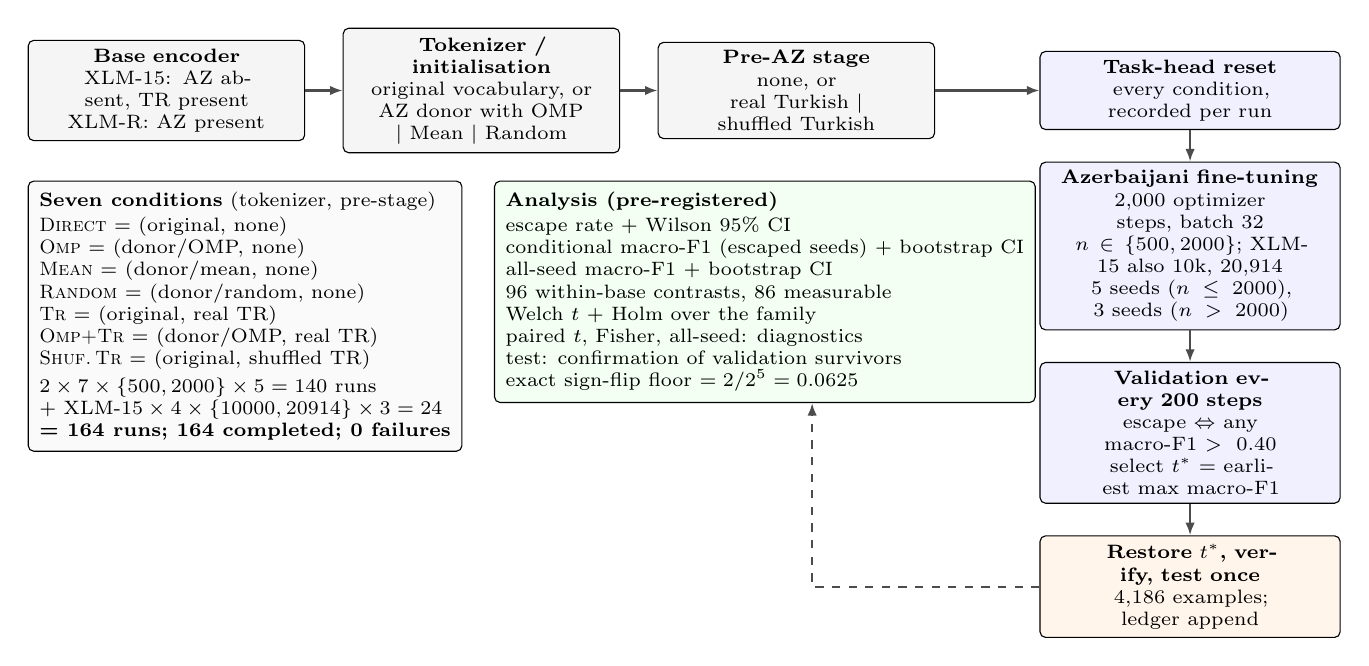
\begin{tikzpicture}[
  font=\scriptsize,
  box/.style={draw, rounded corners=2pt, inner sep=3pt, align=center, fill=white},
  fac/.style={box, fill=black!4, text width=3.3cm},
  stage/.style={box, fill=blue!6, text width=3.6cm},
  outbox/.style={box, fill=orange!8, text width=3.6cm},
  info/.style={box, align=left, inner sep=4pt},
  arr/.style={-{Latex[length=1.6mm]}, thick, black!70}
]
% ---------------- top row: factors
\node[fac] (b1) at (0,0) {\textbf{Base encoder}\\ \xlmxv{}: AZ absent, TR present\\ \xlmr{}: AZ present};
\node[fac] (tok) at (4.0,0) {\textbf{Tokenizer / initialisation}\\ original vocabulary, or\\ AZ donor with OMP $\mid$ Mean $\mid$ Random};
\node[fac] (pre) at (8.0,0) {\textbf{Pre-AZ stage}\\ none, or\\ real Turkish $\mid$ shuffled Turkish};
\node[stage] (reset) at (13.0,0) {\textbf{Task-head reset}\\ every condition, recorded per run};
% ---------------- right column: AZ stage chain
\node[stage, below=4mm of reset] (az) {\textbf{Azerbaijani fine-tuning}\\ 2{,}000 optimizer steps, batch 32\\ $n\in\{500, 2000\}$; \xlmxv{} also 10k, 20{,}914\\ 5 seeds ($n\le2000$), 3 seeds ($n>2000$)};
\node[stage, below=4mm of az] (ev) {\textbf{Validation every 200 steps}\\ escape $\Leftrightarrow$ any \Fone{} $>0.40$\\ select $t^\ast$ = earliest max \Fone};
\node[outbox, below=4mm of ev] (test) {\textbf{Restore $t^\ast$, verify, test once}\\ 4{,}186 examples; ledger append};
% ---------------- bottom-left: conditions
\node[info, fill=black!2, anchor=north west] (cond) at ($(b1.south west)+(0,-0.5)$) {%
\textbf{Seven conditions} (tokenizer, pre-stage)\\[1pt]
\Direct{} = (original, none)\\
\OMP{} = (donor/OMP, none)\\
\Mean{} = (donor/mean, none)\\
\Random{} = (donor/random, none)\\
\TR{} = (original, real TR)\\
\OMPTR{} = (donor/OMP, real TR)\\
\ShufTR{} = (original, shuffled TR)\\[2pt]
$2 \times 7 \times \{500,2000\} \times 5 = 140$ runs\\
$+\ \text{\xlmxv{}} \times 4 \times \{10000,20914\} \times 3 = 24$\\
\textbf{= 164 runs; 164 completed; 0 failures}};
% ---------------- bottom-middle: analysis
\node[info, fill=green!5, anchor=north west] (ana) at ($(cond.north east)+(0.4,0)$) {%
\textbf{Analysis (pre-registered)}\\[1pt]
escape rate + Wilson 95\% CI\\
conditional \Fone{} (escaped seeds) + bootstrap CI\\
all-seed \Fone{} + bootstrap CI\\
96 within-base contrasts, 86 measurable\\
Welch $t$ + Holm over the family\\
paired $t$, Fisher, all-seed: diagnostics\\
test: confirmation of validation survivors\\
exact sign-flip floor $= 2/2^5 = 0.0625$};
% ---------------- arrows
\draw[arr] (b1) -- (tok);
\draw[arr] (tok) -- (pre);
\draw[arr] (pre) -- (reset);
\draw[arr] (reset) -- (az);
\draw[arr] (az) -- (ev);
\draw[arr] (ev) -- (test);
\draw[arr, dashed] (test.west) -| ($(ana.south)+(0.6,0)$);
\end{tikzpicture}
}
\caption{Experimental design. Each run is a triple (base, condition, seed) at one Azerbaijani training size $n$; a condition is a pair (tokenizer/initialisation, pre-Azerbaijani stage). Every arm passes through the same task-head reset, the same 2{,}000-step Azerbaijani budget, the same validation cadence and selection rule, and exactly one test evaluation of the restored selected checkpoint. Counts are from the frozen configuration (\file{evidence/preregistration/FROZEN.md}) and the launcher record (\file{results/launcher\_state.json}).}
\label{fig:design}
\end{figure*}

\subsection{Notation}
Let $\mathcal{B}=\{\text{\xlmxv},\text{\xlmr}\}$ be the base encoders, each with an original tokenizer $\tau_B$ and input-embedding matrix $\mathbf{E}_B\in\mathbb{R}^{V_B\times d_B}$ ($V_B=95{,}000,\ d_B=1024$ for \xlmxv; $V_B=250{,}002,\ d_B=768$ for \xlmr). The donor is the HPLT Azerbaijani BERT with tokenizer $\tau_D$ and embeddings $\mathbf{E}_D\in\mathbb{R}^{V_D\times d_D}$, $V_D=32{,}770$. A \emph{condition} $c=(\kappa,\pi)$ combines a tokenizer/initialisation choice $\kappa\in\{$original, donor/OMP, donor/mean, donor/random$\}$ with a pre-Azerbaijani stage $\pi\in\{$none, real TR, shuffled TR$\}$. Seven of the twelve combinations were run (Table~\ref{tab:conditions}); the remaining five (placebo initialisers with a Turkish stage, and donor tokenizer with shuffled Turkish) were frozen out of scope before the grid to keep the run count inside the compute budget, and their absence is listed as a limitation. A run is $(B,c,n,s)$ with Azerbaijani training size $n$ and seed $s$.

\begin{table}[!t]
\caption{The seven conditions. Ids and names are those of \file{configs/experiment.yaml}; ``sizes'' lists the Azerbaijani training sizes at which the condition was run for each base.}
\label{tab:conditions}
\centering
\scriptsize
\setlength{\tabcolsep}{2.5pt}
\begin{tabular}{@{}lllll@{}}
\toprule
Short & Config name (id) & Init.$^{b}$ & Pre-AZ & Sizes \\
\midrule
\Direct & \pfx{baza} (1) & -- & none & all$^{a}$ \\
\OMP & \pfx{tokenizator} (3) & OMP & none & all$^{a}$ \\
\Mean & \pfx{transplant\_mean} (6) & mean & none & all$^{a}$ \\
\Random & \pfx{transplant\_random\_coef} (7) & random & none & all$^{a}$ \\
\TR & \pfx{turk} (2) & -- & real TR & 500, 2000 \\
\OMPTR & \pfx{her\_ikisi} (4) & OMP & real TR & 500, 2000 \\
\ShufTR & \pfx{turk\_qarisiq} (5) & -- & shuf.\ TR & 500, 2000 \\
\bottomrule
\multicolumn{5}{@{}p{8.6cm}@{}}{$^{a}$\xlmxv: 500, 2000, 10000, 20914; \xlmr: 500, 2000. $^{b}$``--'' keeps the original tokenizer; the other three install the AZ donor tokenizer initialised by OMP ($k{=}64$), the mean of the $k$ nearest anchors, or random coefficients (seed 0).}
\end{tabular}
\end{table}

\subsection{Estimands}
\label{sec:problem:estimands}
Let $F(t)$ denote validation \Fone{} of a run at optimizer step $t\in\mathcal{T}=\{200,400,\dots,2000\}$. A constant predictor on the balanced binary validation split scores $F=1/3$; we call this the \emph{collapse basin}. A run \emph{escapes} if
\begin{equation}
E=\mathbf{1}\!\left[\max_{t\in\mathcal{T}}F(t)>\theta\right],\qquad \theta=0.40,
\label{eq:escape}
\end{equation}
where $\theta$ was fixed from pilot runs and hash-locked before the grid. The selected checkpoint is the earliest maximiser
\begin{equation}
t^{\ast}=\min\big\{t\in\mathcal{T}: F(t)=\max_{t'}F(t')\big\},
\label{eq:select}
\end{equation}
and every run reports $F_{\mathrm{val}}=F(t^{\ast})$ and, after restoring and numerically verifying the checkpoint, $F_{\mathrm{test}}$ on the fixed test split. For a cell (base, condition, $n$) with seeds $\mathcal{S}$ we report three quantities that answer different questions and are never pooled:
\begin{align}
\hat p_{\mathrm{esc}} &= \tfrac{1}{|\mathcal{S}|}\textstyle\sum_{s\in\mathcal{S}}E_s, \label{eq:pesc}\\
\bar F_{\mathrm{cond}} &= \tfrac{1}{\sum_s E_s}\textstyle\sum_{s\in\mathcal{S}}E_s\,F_s, \label{eq:fcond}\\
\bar F_{\mathrm{all}} &= \tfrac{1}{|\mathcal{S}|}\textstyle\sum_{s\in\mathcal{S}}F_s. \label{eq:fall}
\end{align}
$\bar F_{\mathrm{cond}}$ describes predictive quality \emph{given} that optimisation succeeded; it is a selection on outcome and can compare disjoint survivor sets across conditions. $\bar F_{\mathrm{all}}$ charges every collapsed seed at its actual score and is the quantity a practitioner would experience without re-running seeds. \Fone{} is the unweighted mean of the per-class F1 scores,
\begin{equation}
\text{\Fone}=\tfrac12\sum_{y\in\{0,1\}}\frac{2\,\mathrm{TP}_y}{2\,\mathrm{TP}_y+\mathrm{FP}_y+\mathrm{FN}_y}.
\label{eq:macrof1}
\end{equation}

\subsection{Hypotheses as contrasts, and what they identify}
\label{sec:problem:identification}
Each hypothesis maps to within-base contrasts on the estimands above. Table~\ref{tab:identification} states, for each contrast, what changes jointly and therefore what the contrast can and cannot isolate. Cross-base comparisons are descriptive only: the two encoders differ in architecture, non-embedding capacity (151.7M vs.\ 86.0M parameters), and pretraining coverage, so a difference between bases cannot be attributed to Azerbaijani pretraining exposure alone.

\begin{table}[!t]
\caption{Identification map: what each pre-registered contrast changes jointly and what it can therefore support. ``Isolates'' is intentionally strict.}
\label{tab:identification}
\centering
\footnotesize
\begin{tabular}{@{}L{1.75cm}L{2.55cm}L{3.75cm}@{}}
\toprule
Contrast & Jointly changed & Supports / does \emph{not} isolate \\
\midrule
\Direct\ $\to$ \OMP & vocabulary, segmentation, embedding rows, tied output rows, truncation, parameter count & net effect of the implemented transplant pipeline; \emph{not} tokenizer quality vs.\ embedding quality \\
\OMP\ $\to$ \Mean, \OMP\ $\to$ \Random & only the coefficient solver on the same donor vocabulary and anchors & whether the fitted sparse solve beats a crude or random weighting; \emph{not} whether any initialiser is adequate \\
\Direct\ $\to$ \TR & source-task exposure, extra optimisation, lexical overlap, word order & net effect of Turkish intermediate training; \emph{not} its mechanism \\
\ShufTR\ $\to$ \TR & word order, fluency, source-task difficulty (multiset and labels preserved) & order-sensitive component (H1); \emph{not} syntax alone \\
\Direct\ $\to$ \ShufTR & source exposure without natural order & lexical/optimisation component under a degraded source task \\
\OMP\ $\to$ \OMPTR, \TR\ $\to$ \OMPTR & interaction of transplant and Turkish stage & whether the transplant offsets the Turkish outcome; \emph{not} whether Turkish knowledge transferred through donor rows \\
\xlmxv{} vs.\ \xlmr & architecture, capacity, pretraining coverage, tokenizer scheme & descriptive contrast for H2; \emph{not} the effect of Azerbaijani pretraining exposure \\
\bottomrule
\end{tabular}
\end{table}

\section{Method}
\label{sec:method}

\subsection{Base encoders and donor}
\label{sec:method:models}
Table~\ref{tab:models} lists the three models. The primary encoder is the 15-language XLM MLM+TLM checkpoint fine-tuned on XNLI (\file{FacebookAI/xlm-mlm-tlm-xnli15-1024}), whose documented pretraining languages include Turkish but not Azerbaijani; it uses a 95k fastBPE vocabulary with lower-casing and accent removal, which is why its vocabulary contains no token with the letters ş, ç, ö, ü or ğ (Section~\ref{sec:res:tokenizer}). The contrast encoder is \file{xlm-roberta-base}, pretrained on 100 languages including Azerbaijani with a 250k SentencePiece vocabulary. The donor is \file{HPLT/hplt\_bert\_base\_az}, pinned at revision \pfx{a126552c3073}, a byte-level SentencePiece model with 32{,}770 tokens trained on Azerbaijani.

Total parameter counts conflate the vocabulary-dependent embedding table with the vocabulary-independent encoder, so we decompose them. Transplantation leaves every encoder layer, attention and feed-forward weight, layer norm, and (for \xlmxv) position and language embedding bit-for-bit unchanged; the 25.6\% and 60.0\% total-parameter reductions are entirely the smaller embedding table. The two \emph{encoders} are not capacity-matched (151.7M vs.\ 86.0M non-embedding parameters, a $1.8\times$ factor), which is one reason cross-base contrasts are descriptive.

\begin{table}[!t]
\caption{Models. Parameter counts measured from the loaded architectures (\file{HANDOFF.md} §14); embedding parameters are the input token table only.}
\label{tab:models}
\centering
\scriptsize
\setlength{\tabcolsep}{3pt}
\begin{tabular}{@{}L{2.75cm}R{1.85cm}R{1.85cm}R{1.85cm}@{}}
\toprule
 & \xlmxv & \xlmr & AZ donor \\
\midrule
Hugging Face id & \pfx{xlm-mlm-tlm-}\newline\pfx{xnli15-1024} & \pfx{xlm-roberta-}\newline\pfx{base} & \pfx{HPLT/hplt\_}\newline\pfx{bert\_base\_az} \\
Role & primary & contrast & donor \\
Azerbaijani in pretraining & no & yes & yes (only) \\
Turkish in pretraining & yes & yes & no \\
Tokenizer scheme & fastBPE & SentencePiece & SentencePiece, byte \\
Vocabulary & 95{,}000 & 250{,}002 & 32{,}770 \\
Hidden size & 1024 & 768 & 768 \\
Embedding params (original) & 97{,}280{,}000 & 192{,}001{,}536 & -- \\
Embedding params (transplanted) & 33{,}556{,}480 & 25{,}167{,}360 & -- \\
Non-embedding params & 151{,}698{,}434 & 86{,}043{,}650 & -- \\
Total (original / transplanted) & 249.0M / 185.3M & 278.0M / 111.2M & -- \\
Licence & CC-BY-NC-4.0 & MIT & Apache-2.0 \\
\bottomrule
\end{tabular}
\end{table}

\subsection{Anchor identification}
\label{sec:method:anchors}
Transplantation needs a set of \emph{anchors}: donor tokens that also exist in the base vocabulary, so that their donor- and base-space embeddings are both available. Three identification modes were measured (Table~\ref{tab:anchors}). \emph{Strict} intersects canonical token strings including word-boundary markers; \emph{surface} intersects boundary-stripped strings and can mis-pair a word-final donor piece with a word-initial base piece; \emph{functional}, the pre-registered default, asks the base tokenizer itself. For each donor token $v$ with stripped surface $\sigma(v)$,
\begin{equation}
\mathcal{A}=\Big\{(v,u):\ \mathrm{enc}_{\tau_B}(\sigma(v))=\langle u\rangle,\ u\notin\mathcal{U}_B\Big\},
\label{eq:anchor}
\end{equation}
where $\mathrm{enc}_{\tau_B}$ encodes without special tokens and $\mathcal{U}_B$ is the set of unknown and special ids. The exclusion of $\mathcal{U}_B$ matters: a surface the base tokenizer cannot represent encodes to exactly one token, \pfx{<unk>}, and without the exclusion such pairs would bind donor rows to the UNK vector and pull every reconstruction toward it (Amendment~8.2 in the frozen specification). The standalone surface is tried first, then the surface with a leading space; both variants are counted, and in the final evidence all matches were standalone. Algorithm~\ref{alg:anchors} states the procedure. Seven special-token rows are aligned separately and added to the anchor set at installation time, giving 8{,}054 and 9{,}783 mapped rows for 8{,}047 and 9{,}776 lexical anchors.

\begin{table*}[!t]
\caption{Anchor identification. Counts from \file{results/anchors.json}; ``naive'' is the raw string intersection before canonicalisation; share is functional anchors over the donor vocabulary of 32{,}770; ``unfamiliar'' tokens receive reconstructed embeddings.}
\label{tab:anchors}
\centering
\footnotesize
\begin{tabular}{@{}llrrrrrrr@{}}
\toprule
Base & Scheme & $V_B$ & Naive & Strict & Surface & Functional & Share (\%) & Unfamiliar \\
\midrule
% AUTO-GENERATED by report/ieee/tables/make_tables.py -- do not edit by hand.
% source: results/anchors.json
XLM-15 & fastbpe & 95,000 & 1,545 & 1,637 & 3,938 & 8,047 & 24.56 & 24,723 \\
XLM-R & sentencepiece & 250,002 & 2,856 & 10,662 & 9,539 & 9,776 & 29.83 & 22,994 \\
\bottomrule

\end{tabular}
\end{table*}

\begin{algorithm}[!t]
\caption{Functional anchor identification (\file{src/tokenization/anchor\_map.py})}
\label{alg:anchors}
\KwIn{base tokenizer $\tau_B$ with invalid ids $\mathcal{U}_B=\{\mathrm{unk}\}\cup\mathrm{special}$; donor vocabulary $\{(v,\text{str}_v)\}$}
\KwOut{anchor pairs $\mathcal{A}$; unfamiliar donor ids $\mathcal{V}_{\mathrm{unf}}$}
$\mathcal{A}\leftarrow\emptyset$\;
\ForEach{donor id $v$ in ascending order}{
  $\sigma\leftarrow$ decoded surface of $\text{str}_v$, boundary marker stripped\;
  \lIf{$\sigma=\varnothing$}{\textbf{continue}}
  \ForEach{$x\in(\sigma,\ \text{``\textvisiblespace''}\!+\!\sigma)$}{
    $\mathbf{u}\leftarrow\mathrm{enc}_{\tau_B}(x)$ without special tokens\;
    \If{$|\mathbf{u}|=1$ \KwSty{and} $u_1\notin\mathcal{U}_B$}{
      $\mathcal{A}\leftarrow\mathcal{A}\cup\{(v,u_1)\}$; \textbf{break}\;
    }
  }
}
$\mathcal{V}_{\mathrm{unf}}\leftarrow\{v: (v,\cdot)\notin\mathcal{A}\}\setminus\mathrm{special}$\;
\Return{$\mathcal{A},\ \mathcal{V}_{\mathrm{unf}}$}
\end{algorithm}

\subsection{OMP embedding reconstruction and coefficient transfer}
\label{sec:method:omp}
Let $\mathbf{D}_{\mathcal{A}}\in\mathbb{R}^{|\mathcal{A}|\times d_D}$ and $\mathbf{B}_{\mathcal{A}}\in\mathbb{R}^{|\mathcal{A}|\times d_B}$ hold the donor- and base-space embeddings of the anchors, with $\tilde{\mathbf{d}}_a=\mathbf{d}_a/\|\mathbf{d}_a\|_2$ the $\ell_2$-normalised donor rows. For an unfamiliar donor token $v$ with normalised embedding $\tilde{\mathbf{d}}_v$, the candidate set is the $m=256$ anchors with the highest donor-space cosine similarity, sorted in decreasing order,
\begin{equation}
\mathcal{C}(v)=\operatorname{top}_{m}\big\{a\in\mathcal{A}:\ \tilde{\mathbf{d}}_v^{\top}\tilde{\mathbf{d}}_a\big\},
\label{eq:candidates}
\end{equation}
and the coefficients solve the $k$-sparse least-squares problem
\begin{equation}
\bm{\alpha}_v=\arg\min_{\bm{\alpha}\in\mathbb{R}^{m}}\big\|\tilde{\mathbf{d}}_v-\tilde{\mathbf{D}}_{\mathcal{C}(v)}^{\top}\bm{\alpha}\big\|_2^2\quad\text{s.t.}\quad\|\bm{\alpha}\|_0\le k,\ k=64,
\label{eq:omp}
\end{equation}
approximately, by orthogonal matching pursuit \cite{pati1993omp,tropp2007omp} (scikit-learn's \pfx{OrthogonalMatchingPursuit}, no intercept). The coefficients, not the vector, are transferred: the base-space row is
\begin{equation}
\hat{\mathbf{b}}_v=\sum_{a\in\mathcal{C}(v)}\alpha_{v,a}\,\mathbf{b}_a ,
\label{eq:transfer}
\end{equation}
using the \emph{unnormalised} base anchor rows, so that $\hat{\mathbf{b}}_v$ lives on the base model's own scale and $d_D\neq d_B$ is permitted. Restricting to $m=256<d_D=768$ keeps the dictionary undercomplete, which the implementation warns is required for greedy selection to be reliable. The candidate sorting in \eqref{eq:candidates} is what makes the mean placebo below well defined (Amendment~8.1).

\subsection{Placebo initialisers and norm rescaling}
\label{sec:method:placebo}
Two placebos use the same donor vocabulary, anchors, and candidate sets but replace the solver:
\begin{align}
\alpha^{\mathrm{mean}}_{v,a}&=\tfrac{1}{k}\,\mathbf{1}\big[a\in\mathcal{N}_k(v)\big], \label{eq:mean}\\
\alpha^{\mathrm{rand}}_{v,a}&=\frac{z_a\,\mathbf{1}[a\in\mathcal{R}_k(v)]}{\sum_{a'\in\mathcal{R}_k(v)}|z_{a'}|},\qquad z_a\sim\mathcal{N}(0,1), \label{eq:random}
\end{align}
where $\mathcal{N}_k(v)$ is the set of the $k$ nearest candidates (the first $k$ of the sorted $\mathcal{C}(v)$) and $\mathcal{R}_k(v)$ is a set of $k$ candidates drawn uniformly without replacement from $\mathcal{C}(v)$, with one fixed realisation (transplant seed 0). \Mean{} asks whether the fitted sparse solve beats the crudest sensible weighting; \Random{} asks whether \emph{any} placement in the anchor span, with the same sparsity, already delivers whatever benefit the pipeline has. Each transplant artefact is built once; downstream seeds vary fine-tuning only.

A measurement on the raw reconstructions showed that \eqref{eq:transfer} inflates \xlmr{} rows: the median norm of reconstructed rows was $1.9091\times$ that of the base anchor rows (\xlmxv: $1.1324\times$; Section~\ref{sec:res:intrinsic}). Because the pre-registered principle is that reconstructed rows must live at the base model's own scale, every installed artefact, for both bases and all three initialisers, rescales each reconstructed row to the median anchor norm while preserving its direction:
\begin{equation}
\hat{\mathbf{b}}_v\leftarrow\hat{\mathbf{b}}_v\cdot\frac{\operatorname{median}_{a\in\mathcal{A}}\|\mathbf{b}_a\|_2}{\|\hat{\mathbf{b}}_v\|_2}.
\label{eq:rescale}
\end{equation}
The six installed artefacts all report a reconstructed-to-anchor median-norm ratio of exactly 1.000 (Table~\ref{tab:fidelity}).

\subsection{Installing the transplant}
The donor tokenizer replaces the base tokenizer; the input-embedding table is resized to $V_D$ and filled with the anchors' own base rows for $a\in\mathcal{A}$, the aligned special-token rows, and $\hat{\mathbf{b}}_v$ for $v\in\mathcal{V}_{\mathrm{unf}}$; the tied masked-LM output projection receives the same matrix and weights are re-tied. Nothing else in the checkpoint is modified. Algorithm~\ref{alg:transplant} summarises the pipeline.

\begin{algorithm}[!t]
\caption{Tokenizer transplantation (\file{src/transplant/})}
\label{alg:transplant}
\KwIn{$\mathbf{E}_B,\ \mathbf{E}_D$; anchors $\mathcal{A}$; unfamiliar $\mathcal{V}_{\mathrm{unf}}$; method $\in\{$omp, mean, random$\}$; $k{=}64$, $m{=}256$, seed 0}
\KwOut{transplanted checkpoint with donor tokenizer}
$\tilde{\mathbf{D}}_{\mathcal{A}}\leftarrow$ row-normalise $\mathbf{E}_D[\mathcal{A}]$\; $\mathbf{B}_{\mathcal{A}}\leftarrow\mathbf{E}_B[\mathcal{A}]$ (unnormalised)\;
\ForEach{$v\in\mathcal{V}_{\mathrm{unf}}$ \emph{(batches of 256)}}{
  $\tilde{\mathbf{d}}_v\leftarrow\mathbf{E}_D[v]/\|\mathbf{E}_D[v]\|$\;
  $\mathcal{C}(v)\leftarrow$ top-$m$ anchors by $\tilde{\mathbf{d}}_v^{\top}\tilde{\mathbf{d}}_a$, sorted descending\;
  \uIf{method = omp}{$\bm{\alpha}\leftarrow\mathrm{OMP}(\tilde{\mathbf{d}}_v,\tilde{\mathbf{D}}_{\mathcal{C}(v)},k)$ \tcp*[r]{\eqref{eq:omp}}}
  \uElseIf{method = mean}{$\bm{\alpha}\leftarrow\tfrac1k$ on first $k$ candidates \tcp*[r]{\eqref{eq:mean}}}
  \Else{$\bm{\alpha}\leftarrow$ random coefficients on $k$ drawn cand.\ \tcp*[r]{\eqref{eq:random}}}
  $\hat{\mathbf{b}}_v\leftarrow\bm{\alpha}^{\top}\mathbf{B}_{\mathcal{C}(v)}$ \tcp*[r]{coefficient transfer, \eqref{eq:transfer}}
}
$\mathbf{E}'\leftarrow$ resize to $V_D$\; $\mathbf{E}'[a]\leftarrow\mathbf{E}_B[u_a]$ for $(a,u_a)\in\mathcal{A}$; align special rows\; $\mathbf{E}'[v]\leftarrow\hat{\mathbf{b}}_v$ for $v\in\mathcal{V}_{\mathrm{unf}}$\;
rescale each $\mathbf{E}'[v]$ to $\operatorname{median}_a\|\mathbf{E}'[a]\|$ \tcp*[r]{\eqref{eq:rescale}}
install $\mathbf{E}'$ as input table and tied output rows\; save with donor tokenizer\;
run identity, round-trip, forward-pass controls (Sec.~\ref{sec:method:fidelity})\;
\end{algorithm}

\subsection{Fidelity controls}
\label{sec:method:fidelity}
Before any training, each artefact passes controls that rule out serialisation and bookkeeping errors (Table~\ref{tab:fidelity}). The \emph{identity} control maps the base vocabulary onto itself through the same anchor machinery, writes the embedding matrix, saves and reloads the model, and compares a forward pass: the embedding tables are bit-identical after the round trip, the maximum absolute logit difference is $0.0$, and there are no canonical-key collisions. These checks establish that the transplant we evaluated is the transplant we built; they say nothing about whether reconstructed rows carry useful lexical information, which is the subject of the intrinsic diagnostics in Section~\ref{sec:res:intrinsic}.

\begin{table*}[!t]
\caption{Fidelity controls per base (\file{results/controls\_\_\{base\}.json}, \file{results/transplant\_\_\{base\}\_\_*\_rescaled.json}). Ratios are reconstructed-to-anchor median norms of the installed OMP / Mean / Random artefacts after Eq.~\eqref{eq:rescale}.}
\label{tab:fidelity}
\centering
\footnotesize
\begin{tabular}{@{}lcccccl@{}}
\toprule
Base & Identity matrix & Key collisions & Round trip bit-exact & Max $|\Delta\,\mathrm{logit}|$ & Logits identical & Norm ratios OMP / Mean / Random \\
\midrule
% AUTO-GENERATED by report/ieee/tables/make_tables.py -- do not edit by hand.
% source: results/controls__{base}.json (C1a_identity)
% source: results/transplant__{base}__*_rescaled.json (norm_report)
XLM-15 & yes & 0 & yes & 0.0 & yes & 1.000 / 1.000 / 1.000 \\
XLM-R & yes & 0 & yes & 0.0 & yes & 1.000 / 1.000 / 1.000 \\
\bottomrule

\end{tabular}
\end{table*}

\subsection{Turkish intermediate stage and the word-shuffled control}
\label{sec:method:turkish}
Real Turkish training fine-tunes the encoder with a three-class sentiment head on 18{,}000 retained TRSAv1 examples \cite{aydogan2023trsav1} for two epochs, evaluating on 2{,}000 held-out Turkish examples per epoch; its product is the end-of-training checkpoint, built once per (base, tokenizer, corpus, seed)---30 distinct checkpoints, produced serially in a first phase---and reused read-only by the Azerbaijani stage. For \OMPTR{} the Turkish stage runs on the transplanted model, so the Turkish stage itself is affected by the transplant. The shuffled control applies the identical procedure to a corpus in which the whitespace-delimited words of each example are independently permuted, keeping the example's label and word multiset. The manipulation changed word order in 19{,}561 of 20{,}000 examples (97.805\%) and preserved every multiset (\file{results/scramble.json}). Shuffling changes order, fluency, and source-task difficulty together, so real-minus-shuffled is an \emph{order-sensitive} contrast, not a syntax-only intervention.

Source-stage quality is recorded, not assumed: every Turkish-bearing run stores its Turkish validation \Fone{} and a degeneracy flag (\Fone{}$<0.40$ or constant prediction over three classes). Degenerate stages are \emph{reported}, never excluded, because excluding failed source stages would be an outcome-based exclusion.

\subsection{Task-head reset}
\label{sec:method:head}
After the Turkish checkpoint is loaded, every module outside the encoder prefix is re-initialised with the model's own initialiser, for every condition, so that no arm carries a differently aged head: 2{,}050 \pfx{sequence\_summary} parameters for \xlmxv{} and 592{,}130 \pfx{classifier} parameters for \xlmr{}, recorded per run. This closes a defect found by a forensic audit of an earlier grid, in which \pfx{ignore\_mismatched\_sizes} re-initialised only the shape-mismatched output projection and silently carried the Turkish-trained dense projection into the Azerbaijani stage (Amendment~8.3). Consequently any Turkish-stage effect must pass through the encoder.

\subsection{Two-stage training and checkpoint selection}
\label{sec:method:training}
Algorithm~\ref{alg:training} gives the per-run procedure. All Azerbaijani runs use 2{,}000 optimizer steps regardless of $n$, so that update opportunity is held constant: an epoch budget would give roughly 63, 313, 1{,}250 and 6{,}250 steps across the size range and could prevent escape in the small cells by construction. Under the fixed budget the model sees the training subset about 125, 31.7, 6.4 and 3.1 times at $n=500$, 2{,}000, 10{,}000 and 20{,}914 respectively; the size sweep is therefore a fixed-budget stress test, not a converged learning curve. Validation \Fone{} is recorded at every 200 steps; a checkpoint is saved at each evaluation point with \pfx{save\_total\_limit}\,$=1$; the best-by-\Fone{} checkpoint is restored at the end and \emph{re-scored on validation}, and the run aborts if the restored score differs from the recorded maximum by more than $10^{-4}$. Only then is the fixed test split evaluated, once, with predictions stored and an entry appended to a persistent ledger. Early stopping is disabled, so every run trains all 2{,}000 steps and the collapse diagnostics see the full history.

\begin{algorithm}[!t]
\caption{One run $(B,c,n,s)$ (\file{src/training/finetune.py})}
\label{alg:training}
\KwIn{base $B$, condition $c=(\kappa,\pi)$, size $n$, seed $s$; frozen hyperparameters (Table~\ref{tab:hparams})}
set all seeds to $s$; deterministic algorithms on\;
load checkpoint for $\kappa$ (original base, or transplanted artefact of $B$)\;
\If{$\pi\neq$ none}{
  \lIf{cache hit for $(B,s,\pi)$}{load Turkish checkpoint}
  \lElse{train 3-class head on 18k (shuffled) TR, 2 epochs; record TR \Fone; cache}
}
reset every non-encoder module (task head); record what was reset\;
sample $n$ Azerbaijani training examples deterministically for seed $s$\;
\For{$t=1$ \KwTo $2000$}{
  AdamW step: batch 32, lr $2{\cdot}10^{-5}$, warm-up 10\%, wd 0.01, fp16\;
  \If{$t \bmod 200 = 0$}{record $F(t)$ on validation; save checkpoint (keep best)}
}
$E\leftarrow\mathbf{1}[\max_t F(t)>0.40]$; $t^\ast\leftarrow$ earliest argmax \tcp*[r]{Eqs.~\eqref{eq:escape},\eqref{eq:select}}
restore $t^\ast$; re-score validation; \textbf{abort} if $|F_{\text{restored}}-F(t^\ast)|>10^{-4}$\;
evaluate test split once; store predictions; append ledger entry\;
write schema-v4 record (history, selection, test, TR stage, reset, runtime)\;
\end{algorithm}

\subsection{Statistical analysis plan}
\label{sec:method:stats}
All inference is within base and was fixed before the grid. For a cell, the escape count $x$ of $N$ seeds gets a Wilson 95\% interval \cite{wilson1927probable},
\begin{equation}
\frac{\hat p+\frac{z^2}{2N}\pm z\sqrt{\frac{\hat p(1-\hat p)}{N}+\frac{z^2}{4N^2}}}{1+\frac{z^2}{N}},\qquad z=1.96,
\label{eq:wilson}
\end{equation}
and $\bar F_{\mathrm{cond}}$, $\bar F_{\mathrm{all}}$ get 10{,}000-resample percentile bootstrap intervals \cite{efron1993bootstrap}. For a contrast between conditions $A$ and $C$ at the same base and size, escape rates are compared by Fisher's exact test (diagnostic). The \emph{primary family} compares conditional \Fone{} by Welch's $t$ \cite{welch1947generalization},
\begin{equation}
t=\frac{\bar F_C-\bar F_A}{\sqrt{s_C^2/n_C+s_A^2/n_A}},\qquad
\nu=\frac{(s_C^2/n_C+s_A^2/n_A)^2}{\frac{(s_C^2/n_C)^2}{n_C-1}+\frac{(s_A^2/n_A)^2}{n_A-1}},
\label{eq:welch}
\end{equation}
over escaped seeds, and is \emph{measurable} only if both arms have at least two escaped seeds; 86 of the 96 declared contrasts are measurable. The family-wise error is controlled by Holm's step-down rule \cite{holm1979simple}: with ordered raw $p_{(1)}\le\dots\le p_{(M)}$, $M=86$,
\begin{equation}
p^{\mathrm{Holm}}_{(i)}=\max_{j\le i}\min\big\{(M-j+1)\,p_{(j)},\,1\big\},
\label{eq:holm}
\end{equation}
and a contrast \emph{survives} if $p^{\mathrm{Holm}}<0.05$ (the plain Bonferroni threshold is $0.05/86=5.81\times10^{-4}$). Same-seed paired $t$ tests on seeds escaped in both arms, all-seed paired tests, Cohen's $d$, and Fisher tests are reported as diagnostics or sensitivity analyses and are not members of the adjusted family. Test-split inference is restricted to \emph{confirmation}: the 27 validation survivors are re-tested with a paired $t$ on test scores, Holm-corrected within the 27; no new family is discovered on test. Finally, because five paired seeds admit only $2^5=32$ sign assignments, the exact two-sided sign-flip $p$-value \cite{good2005permutation},
\begin{equation}
p_{\mathrm{exact}}=\frac{1}{32}\sum_{\bm{\sigma}\in\{\pm1\}^5}\mathbf{1}\Big[\big|\bar\delta_{\bm{\sigma}}\big|\ge\big|\bar\delta\big|\Big]\ \ge\ \frac{2}{32}=0.0625,
\label{eq:signflip}
\end{equation}
with $\bar\delta_{\bm{\sigma}}=\tfrac15\sum_i\sigma_i\delta_i$ the sign-flipped mean of the five paired seed differences $\delta_i$ and $\bar\delta$ the observed mean,
can never reach $0.05$; parametric survivors are therefore reported as model-based evidence, and \eqref{eq:signflip} is computed for each of them as the distribution-free bound. Algorithm~\ref{alg:stats} summarises the family logic.

\begin{algorithm}[!t]
\caption{Inference family (\file{src/analysis/stats.py})}
\label{alg:stats}
\ForEach{base $B$, size $n$, unordered pair $\{A,C\}$ of conditions run at $(B,n)$}{
  Fisher exact test on escape counts (diagnostic)\;
  \If{$\#\mathrm{esc}(A)\ge2$ \KwSty{and} $\#\mathrm{esc}(C)\ge2$}{
    Welch $t$ on cond.\ \Fone; bootstrap CI; Cohen's $d$ \tcp*[r]{primary family}
  }
  \lElse{mark \textsc{not measured}}
  \lIf{$\ge2$ shared escaped seeds}{paired $t$ (diagnostic)}
  all-seed paired $t$ (sensitivity)\;
}
Holm-adjust the 86 Welch $p$; survivors $\leftarrow\{p^{\mathrm{Holm}}<0.05\}$ \tcp*[r]{\eqref{eq:holm}}
\ForEach{survivor}{paired $t$ on test \Fone; Holm within survivors; exact sign-flip $p$ \tcp*[r]{\eqref{eq:signflip}}}
\end{algorithm}

\section{Experimental Setup}
\label{sec:setup}

\subsection{Azerbaijani task data}
\label{sec:setup:data}
The Azerbaijani source is the LocalDoc sentiment dataset on Hugging Face \cite{localdoc2024sentiment} (42{,}000 texts from social networks and reviews, three classes, licence CC-BY-NC-SA-4.0). The dataset exceeds the brief's floor of 10{,}000 labelled examples; the primary cells at $n\in\{500,2{,}000\}$ are deliberate low-resource subsamples of a fixed training split, chosen because that is where transfer effects are expected and where escape instability was measured in pilots, and the full-size cell $n=20{,}914$ establishes the ceiling. Table~\ref{tab:azdata} traces the pipeline. Neutral examples are removed to obtain a binary task; label-aware exact-text deduplication removes 86 duplicates (0.31\%) with zero label conflicts, \emph{before} a stratified split with seed 12{,}345. The resulting splits are balanced, and an exact-text leakage check finds no overlap between any pair of splits. Because the upstream Hugging Face revision is not pinned, an order-invariant content manifest (SHA-256 over sorted normalised text–label pairs) is recorded for every split; the supplied \file{data.tgz} snapshot is the only exact copy of the data the grid saw, and any reproduction must verify the manifests before treating a fresh download as equivalent. No scraping was performed and no personal data beyond the public dataset was used.

\begin{table}[!t]
\caption{Azerbaijani data pipeline and splits (\file{results/splits.json}). The pre-grid characterisation package (Section~\ref{sec:setup:audit}) used 20{,}936/2{,}791/4{,}187 and carries no manifest.}
\label{tab:azdata}
\centering
\scriptsize
\begin{tabular}{@{}L{5.3cm}R{3.3cm}@{}}
\toprule
Step & Count \\
\midrule
Upstream rows (positive / neutral / negative) & 42{,}000 \\
After removing \pfx{neutral} & 28{,}000 \\
After label-aware exact-text deduplication (86 removed, 0 conflicts) & 27{,}914 \\
Train / validation / test (stratified, seed 12{,}345) & 20{,}937 / 2{,}791 / 4{,}186 \\
Train label distribution (negative / positive) & 10{,}472 / 10{,}465 \\
Test label distribution (negative / positive) & 2{,}094 / 2{,}092 \\
Exact-text leakage train–test / train–val / val–test & 0 / 0 / 0 \\
Content manifest, test split (SHA-256 prefix) & \pfx{ca19c0bb} \\
Content manifest, validation / train (prefix) & \pfx{5cd479fb} / \pfx{d1cf165c} \\
Upstream revision pinned & no \\
\bottomrule
\end{tabular}
\end{table}

\subsection{Human label audit (pre-grid)}
\label{sec:setup:audit}
Two annotators independently labelled 100 examples sampled under the pre-grid split (Table~\ref{tab:audit}). Three-class human–human agreement is 66/99 (66.67\%, $\kappa=0.491$). Among rows retained by the binary task, the \emph{unconditioned} agreement is 44/67 (65.67\%); the higher 37/42 (88.10\%, $\kappa=0.746$) conditions on both humans and the dataset all committing to a polarity and therefore selects easier examples. The unconditioned figure is the relevant disclosure of retained-label quality, and the two annotators are not interchangeable (68.66\% vs.\ 59.70\% against gold). Because the pre-grid split differs from the grid split by one example and has no manifest, these numbers characterise the dataset, not the specific holdout.

\begin{table}[!t]
\caption{Human label audit, 100 sampled examples (\file{evidence/carried\_forward\_pre\_grid/}).}
\label{tab:audit}
\centering
\scriptsize
\begin{tabular}{@{}L{4.5cm}R{4.1cm}@{}}
\toprule
Quantity & Value \\
\midrule
Three-class human–human agreement & 66/99 = 66.67\% ($\kappa$ = 0.491) \\
Human–human on retained polar rows, unconditioned & 44/67 = 65.67\% \\
Human–human, all three sources commit to a polarity & 37/42 = 88.10\% ($\kappa$ = 0.746) \\
Annotator 1 vs.\ gold (100 / retained 67) & 71.0\% / 68.66\% \\
Annotator 2 vs.\ gold (100 / retained 67) & 58.59\% / 59.70\% \\
Audit verdict & \pfx{PROCEED\_WITH\_CAVEAT} \\
\bottomrule
\end{tabular}
\end{table}

\subsection{Turkish source data}
TRSAv1 \cite{aydogan2023trsav1} provides 150{,}000 Turkish e-commerce reviews with three labels; the captured dataset card declares no licence. Label-aware deduplication removes 11{,}360 rows (7.57\%; 937 texts had conflicting labels), leaving 138{,}640, from which a seeded, label-stratified subsample of 20{,}000 is deterministically partitioned into 18{,}000 source-training and 2{,}000 source-validation examples. The shuffled corpus is derived from the same 20{,}000 (Section~\ref{sec:method:turkish}).

\subsection{Pre-registration and amendments}
\label{sec:setup:prereg}
The experimental specification was frozen on 4 September 2026 and hash-locked (\file{configs/CONFIG\_HASHES.lock}); every later change is an amendment recorded with its date and rationale before the affected runs (Table~\ref{tab:prereg}). Two classes of amendment exist. Non-scientific execution changes (validation cadence 65$\to$200 steps, evaluation batch size, two-phase execution, a gradient-accumulation option adopted and then reverted before any run completed) do not alter what the optimizer does at any step. Amendments~6 and~8, written before the final grid, repair defects found by a forensic audit of an earlier 114-run grid: validation-selected checkpoint restoration with numerical verification, a genuinely reset task head, a well-defined mean placebo, UNK-free anchors, degeneracy accounting, dual estimands with family-wise correction, and content manifests. That earlier grid is retained unmodified as a separate artefact and is not pooled with the 164 runs reported here. The escape threshold $\theta=0.40$, the seeds, sizes, $k$, $m$, and every optimizer setting were never changed after the freeze.

\begin{table}[!t]
\caption{Pre-registration timeline (\file{evidence/preregistration/FROZEN.md}).}
\label{tab:prereg}
\centering
\scriptsize
\begin{tabular}{@{}L{1.4cm}L{7.1cm}@{}}
\toprule
Date (2026) & Event \\
\midrule
04 Sep & Specification frozen; hash lock; $\theta=0.40$ fixed from pilots \\
04 Sep & Validation cadence 65 $\to$ 200 steps; eval batch size; A100/H100 migration notes; gradient accumulation $8\times4$ authorised \\
05 Sep & Accumulation reverted to pre-registered batch 32 $\times$ 1 (no run had completed under $8\times4$) \\
06 Sep & 114-run validation-only grid (retained separately, not pooled) \\
07 Sep & Amendments 1–5: Turkish conditions and contrast base at $n=500$; test split spent once with ledger; schema v4; per-method C1c provenance \\
07 Sep & Amendment 6: best-validation checkpoint restore with $10^{-4}$ verification \\
08 Sep & Amendment 8: nearest-$k$ mean placebo; UNK/special rejection in anchors; full task-head reset; degeneracy accounting; all-seed estimand, paired tests, Holm; manifests; valid JSON \\
08–09 Sep & Final 164-run grid executed (19:39 UTC 8 Sep to 03:58 UTC 9 Sep) \\
\bottomrule
\end{tabular}
\end{table}

\subsection{Grid, seeds, and hyperparameters}
\label{sec:setup:grid}
Table~\ref{tab:hparams} lists the frozen values. At $n=500$ and $n=2{,}000$ both encoders run all seven conditions with seeds $\{42, 1337, 13, 7, 2024\}$ (140 runs); \xlmxv{} additionally runs the four non-Turkish conditions at $n\in\{10{,}000, 20{,}914\}$ with seeds $\{42, 1337, 13\}$ (24 runs). The launcher records 164 requested, 164 completed, zero failures, and no skipped-existing records. The queue is ordered reference-size-first so that a truncated window would still yield a complete comparison table.

\begin{table}[!t]
\caption{Frozen hyperparameters and grid composition (\file{configs/experiment.yaml}, \file{FROZEN.md}).}
\label{tab:hparams}
\centering
\scriptsize
\begin{tabular}{@{}L{3.0cm}L{5.5cm}@{}}
\toprule
Setting & Value \\
\midrule
Azerbaijani budget & 2{,}000 optimizer steps (all $n$) \\
Batch / accumulation / effective batch & 32 / 1 / 32 \\
Optimizer & AdamW \cite{loshchilov2019adamw}, lr $2\times10^{-5}$, warm-up 10\%, weight decay 0.01 \\
Precision / max length / padding & fp16 AMP / 256 / dynamic \\
Validation cadence & every 200 steps (10 points incl.\ terminal) \\
Selection rule & max validation \Fone, ties $\to$ lower step; restore and verify ($10^{-4}$) \\
Early stopping & disabled \\
Escape threshold $\theta$ & 0.40 (fixed from pilots, hash-locked) \\
Turkish stage & 2 epochs, 18k train / 2k val, 3 labels, cached (30 checkpoints) \\
Transplant & functional anchors; $k=64$; $m=256$; rescale to anchor median; transplant seed 0 \\
Seeds ($n\le2{,}000$ / $n>2{,}000$) & \{42, 1337, 13, 7, 2024\} / \{42, 1337, 13\} \\
Split seed & 12{,}345 \\
Runs: $2\times7\times2\times5$ + $1\times4\times2\times3$ & 140 + 24 = 164 (164 completed, 0 failed) \\
Determinism & \pfx{use\_deterministic\_algorithms}; cuDNN deterministic \\
\bottomrule
\end{tabular}
\end{table}

\subsection{Test-split protocol and disclosures}
\label{sec:setup:test}
The inference family is defined on validation. The test split is evaluated once per run, only at the restored validation-selected checkpoint, and only after the restore has been numerically verified; the ledger \file{results/test\_evaluation\_ledger.jsonl} holds exactly 164 entries, one per completed run, all from the single call site \file{finetune.run\_single}, which defaults to the validation split and evaluates the test split only with an explicit opt-in flag. No model, step, hyperparameter, or condition was selected using a test number; test-side statements in Section~\ref{sec:results} are confirmations of validation-selected claims (Section~\ref{sec:method:stats}).

\subsection{Compute environment and budget}
\label{sec:setup:compute}
The 164-run grid executed on a rented instance with one NVIDIA H100 NVL (95{,}830~MiB), an AMD EPYC 9V84 (40 vCPU), 313~GiB RAM, driver 595.71 with CUDA 13.2 host and PyTorch 2.11.0+cu128, in a single stream throughout (\pfx{streams\_active}\,$=1$ in all 164 records). Table~\ref{tab:compute} summarises cost: 8.36 process-hours summed over runs, of which 8.02~h is the Azerbaijani stage; launcher wall-clock 8.37~h; roughly 9.5~h including the serial Turkish-cache phase; hence about 9.5 device-hours. Per-run wall-clock is 2.5–6.8 minutes (Fig.~\ref{fig:runtime}). This is far inside the brief's two-day training envelope. Peak GPU memory during the grid is \NM: the launcher's memory sampler did not run, no run record carries a maximum allocation, and the 97~MiB reading captured after completion describes an idle device. A 30-step benchmark at the locked batch and sequence settings on a different, pre-grid machine (RTX 4060 laptop, 8.59~GB) measured 8.6~GB peak reserved memory; we report it as a labelled pre-grid measurement on other hardware, not as the grid's footprint, and note that a stream ceiling of 10~GB was enforced by the launcher configuration on every venue.

\begin{table}[!t]
\caption{Compute cost of the final grid (\file{evidence/environment/ENVIRONMENT\_AS\_RUN.md}, \file{results/aggregate.csv}, \file{results/launcher\_state.json}). Per-run wall-clock in minutes.}
\label{tab:compute}
\centering
\scriptsize
\begin{tabular}{@{}lrrrrr@{}}
\toprule
Base & Runs & Process-h & Mean & Min & Max \\
\midrule
% AUTO-GENERATED by report/ieee/tables/make_tables.py -- do not edit by hand.
% source: results/aggregate.csv
% source: results/launcher_state.json
XLM-15 & 94 & 5.00 & 3.19 & 2.94 & 3.60 \\
XLM-R & 70 & 3.36 & 2.88 & 2.53 & 6.77 \\
\midrule
All & 164 & 8.36 & 3.06 & 2.53 & 6.77 \\
\bottomrule

\end{tabular}
\par\smallskip
\begin{minipage}{\columnwidth}\footnotesize
Azerbaijani-stage process-hours: 8.02; launcher elapsed: 8.37 h; streams: 1. Wall-clock incl.\ the serial Turkish-cache phase $\approx$ 9.5 h $\Rightarrow$ $\approx$ 9.5 GPU-hours on one GPU. Peak GPU memory during the grid: \NM{} (sampler did not run). Pre-grid 30-step benchmark on an RTX 4060 at the same batch and length: 8.6 GB peak reserved.
\end{minipage}
\end{table}

\begin{figure}[!t]
\centering
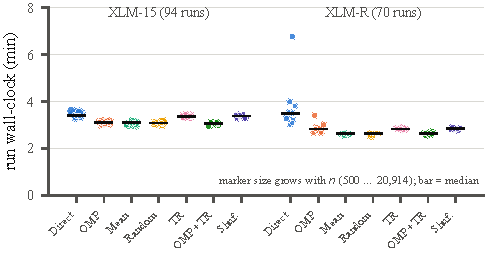
\includegraphics[width=\columnwidth]{figures/fig_runtime.pdf}
\caption{Per-run wall-clock by base and condition, all 164 runs (\file{results/aggregate.csv}). Marker size grows with $n$; the bar is the cell median. Turkish-bearing runs exclude the cached source stage.}
\label{fig:runtime}
\end{figure}

\subsection{Software stack and reproducibility}
\label{sec:setup:repro}
The executed environment used Python 3.12.14, PyTorch 2.11.0+cu128 \cite{paszke2019pytorch}, Transformers 4.57.6 \cite{wolf2020transformers}, Tokenizers 0.22.2, Datasets 5.0.1, NumPy 2.5.3, SciPy 1.18.1, scikit-learn 1.9.0 \cite{pedregosa2011sklearn}, pandas 3.0.5 and Matplotlib 3.11.1 (Table~\ref{tab:stack}). Two disclosures follow from the environment capture. The pre-run \file{requirements.lock} was unresolvable on the host because of a Datasets/fsspec conflict, so it did not describe the run; \pfx{sacremoses} (needed by the \xlmxv{} tokenizer) and \pfx{protobuf} (needed for SentencePiece conversion) were undeclared and installed after import failures. \file{requirements.txt} and \file{requirements.lock} were regenerated from the post-run freeze and describe the environment the reported numbers were computed on; they do not retroactively prove that the original specification was sufficient.

\begin{table}[!t]
\caption{Pre-run pins vs.\ the stack that actually ran (\file{evidence/environment/}).}
\label{tab:stack}
\centering
\scriptsize
\begin{tabular}{@{}lll@{}}
\toprule
Package & Pre-run lock & As run \\
\midrule
torch & 2.4.1+cu121 & 2.11.0+cu128 \\
transformers & 4.44.2 & 4.57.6 \\
tokenizers & 0.19.1 & 0.22.2 \\
datasets & 2.21.0 & 5.0.1 \\
numpy & 1.26.4 & 2.5.3 \\
scipy & 1.14.1 & 1.18.1 \\
scikit-learn & 1.5.2 & 1.9.0 \\
pandas & 2.2.3 & 3.0.5 \\
matplotlib & 3.9.2 & 3.11.1 \\
sentencepiece & 0.2.0 & 0.2.2 \\
sacremoses & 0.2.0 & 0.2.0 (undeclared) \\
protobuf & absent & 7.36.1 (undeclared) \\
\bottomrule
\end{tabular}
\end{table}

All seeds, sizes, paths and analysis rules are read from \file{configs/experiment.yaml}; \file{run\_all.sh} is the single entry point that rebuilds anchors, transplants, controls, the Turkish cache, the 164-run grid, and the aggregate, statistics, and table files in order, with automatic resume through \pfx{skip\_existing}. The repository's continuous-integration workflow (\file{.github/workflows/ci.yml}) runs the CPU unit-test suite (\pfx{pytest -m 'not slow'}, offline, no model or dataset downloads) together with repository-hygiene checks on every push to and pull request against \pfx{main}. Every result file cited in this paper is committed: 164 schema-v4 run records (each with the ten-point validation history, the training-loss history, the test block with all 4{,}186 predictions, the selection and restoration fields, and the task-head-reset and source-stage metadata), the per-run logs, \file{aggregate.csv}, \file{summary.csv}, \file{stats.csv}, the intrinsic-diagnostic and control files, the environment captures, and the pre-registration documents (Appendix~\ref{app:evidence}). Per-run model weights and the 30 Turkish-stage checkpoints are not distributed (tens of GB); their reconstruction costs roughly 2.5 GPU-hours.

\section{Results}
\label{sec:results}

All numbers below are read from the committed result files; the figure and table scripts in \file{report/ieee/} regenerate every artefact from those files. Values are reported to the precision of the source.

\subsection{Tokenizer-level diagnostics}
\label{sec:res:tokenizer}
Fig.~\ref{fig:tokenizer} and Table~\ref{tab:tokenizer} characterise the three tokenizers on 5{,}000 Azerbaijani Wikipedia sentences (102{,}726 words) and on the 27{,}914 task examples. \xlmxv{} segments Azerbaijani into 3.21 tokens per word, \xlmr{} into 1.90, and the donor into 1.76; the \xlmxv{} deficit is structural, because its lower-cased, accent-stripped fastBPE vocabulary contains no token bearing ş, ç, ö, ü or ğ and only two containing ə, whereas \xlmr{} and the donor contain thousands (pre-grid vocabulary counts, \file{diacritics.json}). At the frozen maximum length of 256 tokens, 1.257\% of task examples are truncated under \xlmxv{}, 0.473\% under \xlmr{}, and 0.351\% under the donor; the transplant therefore also changes how much text the encoder sees, a confound of at most 0.9 percentage points of examples.

Alphabetic token-type overlap between Azerbaijani and four other languages (Fig.~\ref{fig:tokenizer}b) shows that Turkish covers more Azerbaijani types than English or Finnish for every vocabulary---66.7\% vs.\ a 58.2\% Latin-script baseline for \xlmxv{} (+8.5~pt), 46.4\% vs.\ 33.8\% for \xlmr{} (+12.6~pt), 32.1\% vs.\ 19.2\% for the donor (+12.9~pt)---while Cyrillic-script Russian covers 8–17\%. The English–Finnish spread is at most 1.6~pt, so the Turkish lift is not noise, but the Russian comparison shows that script alone moves overlap by tens of points; overlap is a lexical-similarity signal, not evidence of linguistic transfer, and it is the reason a lexical-only explanation of any Turkish benefit cannot be excluded by design.

\begin{figure*}[!t]
\centering
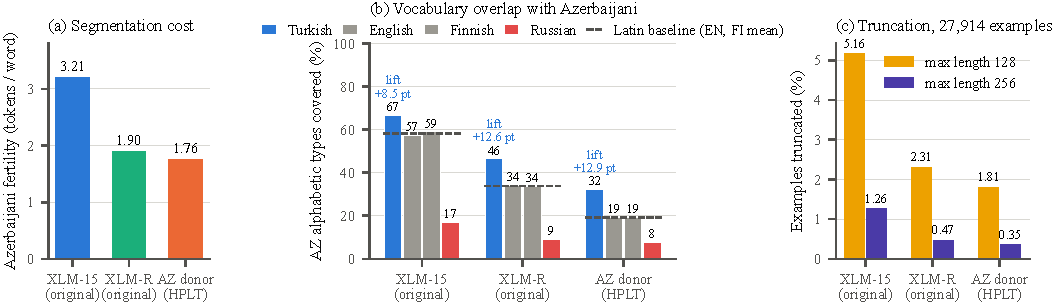
\includegraphics[width=\textwidth]{figures/fig_tokenizer.pdf}
\caption{Tokenizer diagnostics. (a) Azerbaijani fertility on 5{,}000 Wikipedia sentences (\file{results/overlap\_control.json}). (b) Share of Azerbaijani alphabetic token types also present in the tokenization of 5{,}000 sentences of Turkish, English, Finnish and Russian; the dashed line is the English–Finnish mean, the annotated lift is Turkish minus that baseline. (c) Share of the 27{,}914 task examples truncated at maximum length 128 and 256 (\file{results/truncation.json}); 256 is the frozen setting.}
\label{fig:tokenizer}
\end{figure*}

\begin{table*}[!t]
\caption{Tokenizer diagnostics. Fertility, alphabetic types and overlap from \file{results/overlap\_control.json} (5{,}000 Wikipedia sentences per language); letter counts are the number of vocabulary entries containing the letter (\file{evidence/carried\_forward\_pre\_grid/diacritics.json}, pre-grid, dataset-level); token-length statistics and truncation from \file{results/truncation.json} on the 27{,}914 task examples. Lift = Turkish overlap minus the English–Finnish mean.}
\label{tab:tokenizer}
\centering
\footnotesize
\begin{tabular}{@{}lrrrrrrrrrrrrrrr@{}}
\toprule
 & & & AZ alpha. & \multicolumn{4}{c}{AZ types covered by (\%)} & & \multicolumn{3}{c}{Vocab.\ entries with} & \multicolumn{2}{c}{Task tokens} & \multicolumn{2}{c}{Truncated (\%)} \\
\cmidrule(lr){5-8}\cmidrule(lr){10-12}\cmidrule(lr){13-14}\cmidrule(lr){15-16}
Tokenizer & Vocab & Fertility & types & TR & EN & FI & RU & Lift & ə & ş & ğ & mean & p99 & 128 & 256 \\
\midrule
% AUTO-GENERATED by report/ieee/tables/make_tables.py -- do not edit by hand.
% source: results/overlap_control.json
% source: results/truncation.json
% source: evidence/carried_forward_pre_grid/diacritics.json (pre-grid vocabulary letter counts)
XLM-15 & 95,000 & 3.206 & 3,257 & 66.7 & 57.4 & 59.0 & 16.8 & +8.5 & 2 & 0 & 0 & 49.0 & 283 & 5.16 & 1.26 \\
XLM-R & 250,002 & 1.904 & 10,054 & 46.4 & 34.1 & 33.6 & 9.0 & +12.6 & 1,366 & 891 & 407 & 33.7 & 189 & 2.31 & 0.47 \\
AZ donor & 32,770 & 1.758 & 14,858 & 32.1 & 19.3 & 19.1 & 7.7 & +12.9 & 8,814 & 2,253 & 928 & 30.3 & 169 & 1.81 & 0.35 \\
\bottomrule

\end{tabular}
\end{table*}

\subsection{Intrinsic transplant diagnostics}
\label{sec:res:intrinsic}
Before any downstream training, each transplanted artefact was probed on a deterministic 300-line sample of Azerbaijani \emph{training} text (validation and test untouched) with three intrinsic measures (Table~\ref{tab:intrinsic}, Fig.~\ref{fig:intrinsic}): masked-token top-1 accuracy of the masked-LM head, bits per character (BPC), and the embedding-norm ratio before rescaling. BPC rather than perplexity is used because different tokenizers split the same text into different numbers of tokens; BPC normalises the masked-LM loss by characters:
\begin{equation}
\mathrm{BPC}=\frac{\ell_{\mathrm{MLM}}\cdot N_{\mathrm{tok}}}{N_{\mathrm{char}}\ln 2},
\label{eq:bpc}
\end{equation}
with $\ell_{\mathrm{MLM}}$ the mean loss per masked token in nats.

The two bases behave very differently. \xlmr{}'s original masked-LM head predicts 602 of 1{,}631 masked Azerbaijani tokens (36.91\%) at 1.60 BPC; after OMP transplantation it predicts 40 of 1{,}502 (2.66\%) at 6.94 BPC ($\Delta=+5.34$), and the raw reconstruction inflated row norms by $1.91\times$ before rescaling, outside the healthy band of $[0.85, 1.15]$ defined in the norm report. The placebos are worse still ($\Delta$BPC $+5.53$ for \Mean{}, $+7.06$ for \Random{}), so OMP is the \emph{best} of the three initialisers on \xlmr{} while remaining far from the original. \xlmxv{}'s original head is already near chance on Azerbaijani (2 of 2{,}323, 0.09\%; 7.21 BPC), and its OMP transplant stays at 2 of 1{,}502 with a \emph{lower} BPC of 6.00 ($\Delta=-1.20$) and a healthy norm ratio of 1.13. As the quality file itself warns, a BPC decrease at near-zero top-1 accuracy is a calibration change over a smaller vocabulary, not recovered lexical knowledge; the two measures must be read together. Eligible masked positions differ between tokenizers, so these are diagnostics rather than paired token-level accuracies. The independent signals---top-1 collapse, BPC increase, and norm inflation---all point to the same conclusion the downstream grid reaches for \xlmr{}: the implemented reconstruction does not preserve the information the encoder expects in its embedding rows.

\begin{table*}[!t]
\caption{Intrinsic diagnostics of the installed artefacts on 300 Azerbaijani training lines (\file{results/controls\_\_\{base\}\_\_\{tag\}.json}). Top-1 is correct/masked positions; BPC per Eq.~\eqref{eq:bpc}; the norm ratio is reconstructed-to-anchor median norm of the raw OMP reconstruction \emph{before} Eq.~\eqref{eq:rescale} (\file{embedding\_norm\_report}); all installed artefacts are rescaled to 1.000.}
\label{tab:intrinsic}
\centering
\footnotesize
\begin{tabular}{@{}llrrrrrr@{}}
\toprule
 & & \multicolumn{2}{c}{Top-1 (correct/masked)} & \multicolumn{3}{c}{BPC} & Pre-rescale \\
\cmidrule(lr){3-4}\cmidrule(lr){5-7}
Base & Init. & original & transplanted & original & transpl. & $\Delta$ & norm ratio \\
\midrule
% AUTO-GENERATED by report/ieee/tables/make_tables.py -- do not edit by hand.
% source: results/controls__{base}__{tag}.json (C1c)
% source: results/embedding_norm_report__{base}.json (pre-rescale norm ratio)
XLM-15 & OMP & 2/2,323 & 2/1,502 & 7.2071 & 6.0034 & -1.2037 & 1.1324 \\
XLM-15 & Mean & 2/2,323 & 0/1,502 & 7.2071 & 6.0763 & -1.1308 & -- \\
XLM-15 & Random & 2/2,323 & 6/1,502 & 7.2071 & 8.1814 & +0.9743 & -- \\
\midrule
XLM-R & OMP & 602/1,631 & 40/1,502 & 1.5975 & 6.9352 & +5.3377 & 1.9091 \\
XLM-R & Mean & 602/1,631 & 19/1,502 & 1.5975 & 7.1276 & +5.5301 & -- \\
XLM-R & Random & 602/1,631 & 16/1,502 & 1.5975 & 8.6611 & +7.0636 & -- \\
\bottomrule

\end{tabular}
\end{table*}

\begin{figure*}[!t]
\centering
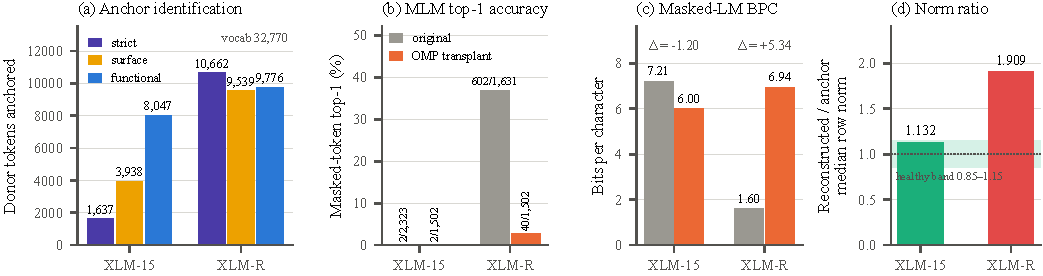
\includegraphics[width=\textwidth]{figures/fig_intrinsic.pdf}
\caption{Intrinsic transplant diagnostics. (a) Anchors found by the three identification modes (\file{results/anchors.json}); functional mode is the pre-registered default. (b) Masked-token top-1 accuracy of the original and the OMP-transplanted masked-LM head on the same 300 training lines (\file{results/top1\_accuracy.json}). (c) Bits per character (\file{results/cross\_base\_transplant\_quality.json}). (d) Reconstructed-to-anchor median-norm ratio of the raw OMP reconstruction with the healthy band of the norm report (\file{results/embedding\_norm\_report\_\_*.json}); the installed artefacts were rescaled to 1.000.}
\label{fig:intrinsic}
\end{figure*}

\subsection{Reference-size grid}
\label{sec:res:grid}
Tables~\ref{tab:results2000} and~\ref{tab:results500} report every cell at the two primary sizes on validation and on test; Appendix~\ref{app:cells} adds the confidence intervals and the higher-data cells. Two facts organise everything that follows. First, \xlmr{} escapes in every one of its 70 runs, so its conditional and all-seed estimands coincide and every \xlmr{} contrast is measurable. Second, \xlmxv{} escapes in 60 of 94 runs, between 2/5 and 5/5 per cell at the primary sizes, so its two estimands diverge by up to 0.21 and its conditional means describe different survivor subsets in different conditions.

For \xlmr{} at $n=2{,}000$, \OMP{} minus \Direct{} is $-0.0659$ on validation (0.8277$\to$0.7618) and $-0.0566$ on test (0.7970$\to$0.7404); at $n=500$ the effects are $-0.0782$ and $-0.0748$. \Mean{} ($-0.0505$, $-0.0560$) and \Random{} ($-0.0980$, $-0.0996$) also underperform \Direct{} at both sizes, with \Random{} worst, and \OMP{} sits between them: better than \Random{} by $+0.032$ and $+0.021$, worse than \Mean{} by $-0.016$ and $-0.022$. \TR{} is the numerically best \xlmr{} condition at both sizes (0.8307 and 0.8149 on validation; 0.8048 and 0.7910 on test), followed by \ShufTR{} and \Direct{}; \OMPTR{} lies between \OMP{} and \Mean{}. For \xlmxv{}, conditional means at $n=2{,}000$ lie within 0.61–0.70 for every condition while all-seed means range from 0.48 (\Direct, 2/5 escaped) to 0.67 (\OMPTR, 5/5); the ordering of conditions depends on which estimand is chosen.

\begin{table*}[!t]
\caption{Complete results at $n=2{,}000$. Escape is escaped/declared seeds; conditional \Fone{} averages escaped seeds only (10{,}000-resample percentile bootstrap 95\% CI); all-seed \Fone{} charges collapsed seeds at their actual score; test values are from the restored validation-selected checkpoint; TR deg.\ counts degenerate Turkish source stages (\file{results/summary.csv}, T1 of \file{evidence/supplemental/test\_tables\_received.md}).}
\label{tab:results2000}
\centering
\footnotesize
\begin{tabular}{@{}llcrlrrrc@{}}
\toprule
 & & & \multicolumn{3}{c}{Validation \Fone} & \multicolumn{2}{c}{Test \Fone} & \\
\cmidrule(lr){4-6}\cmidrule(lr){7-8}
Base & Condition & Escape & cond. & 95\% CI & all-seed & cond. & all-seed & TR deg. \\
\midrule
% AUTO-GENERATED by report/ieee/tables/make_tables.py -- do not edit by hand.
% source: results/summary.csv
% source: evidence/supplemental/test_tables_received.md (T1)
% source: results/runs/*.json
XLM-15 & Direct & 2/5 & 0.6791 & [0.674, 0.684] & 0.4799 & 0.6735 & 0.4790 & 0 \\
XLM-15 & OMP & 3/5 & 0.6148 & [0.464, 0.691] & 0.5023 & 0.6076 & 0.4980 & 0 \\
XLM-15 & Mean & 3/5 & 0.6955 & [0.675, 0.706] & 0.5507 & 0.6833 & 0.5434 & 0 \\
XLM-15 & Random & 4/5 & 0.6699 & [0.664, 0.673] & 0.6026 & 0.6529 & 0.5890 & 0 \\
XLM-15 & TR & 4/5 & 0.6747 & [0.661, 0.687] & 0.6064 & 0.6663 & 0.5997 & 2 \\
XLM-15 & OMP+TR & 5/5 & 0.6712 & [0.645, 0.689] & 0.6712 & 0.6645 & 0.6645 & 3 \\
XLM-15 & Shuf. TR & 2/5 & 0.6873 & [0.682, 0.692] & 0.4750 & 0.6784 & 0.4714 & 2 \\
\midrule
XLM-R & Direct & 5/5 & 0.8277 & [0.823, 0.833] & 0.8277 & 0.7970 & 0.7970 & 0 \\
XLM-R & OMP & 5/5 & 0.7618 & [0.755, 0.769] & 0.7618 & 0.7404 & 0.7404 & 0 \\
XLM-R & Mean & 5/5 & 0.7772 & [0.772, 0.783] & 0.7772 & 0.7578 & 0.7578 & 0 \\
XLM-R & Random & 5/5 & 0.7297 & [0.725, 0.735] & 0.7297 & 0.7154 & 0.7154 & 0 \\
XLM-R & TR & 5/5 & 0.8307 & [0.829, 0.832] & 0.8307 & 0.8048 & 0.8048 & 0 \\
XLM-R & OMP+TR & 5/5 & 0.7708 & [0.766, 0.776] & 0.7708 & 0.7546 & 0.7546 & 0 \\
XLM-R & Shuf. TR & 5/5 & 0.8269 & [0.825, 0.829] & 0.8269 & 0.7971 & 0.7971 & 0 \\
\bottomrule

\end{tabular}
\end{table*}

\begin{table*}[!t]
\caption{Complete results at $n=500$; columns as in Table~\ref{tab:results2000}.}
\label{tab:results500}
\centering
\footnotesize
\begin{tabular}{@{}llcrlrrrc@{}}
\toprule
 & & & \multicolumn{3}{c}{Validation \Fone} & \multicolumn{2}{c}{Test \Fone} & \\
\cmidrule(lr){4-6}\cmidrule(lr){7-8}
Base & Condition & Escape & cond. & 95\% CI & all-seed & cond. & all-seed & TR deg. \\
\midrule
% AUTO-GENERATED by report/ieee/tables/make_tables.py -- do not edit by hand.
% source: results/summary.csv
% source: evidence/supplemental/test_tables_received.md (T1)
% source: results/runs/*.json
XLM-15 & Direct & 3/5 & 0.6306 & [0.621, 0.639] & 0.5117 & 0.6229 & 0.5071 & 0 \\
XLM-15 & OMP & 2/5 & 0.5272 & [0.440, 0.614] & 0.4109 & 0.5248 & 0.4100 & 0 \\
XLM-15 & Mean & 2/5 & 0.6359 & [0.627, 0.645] & 0.4544 & 0.6302 & 0.4521 & 0 \\
XLM-15 & Random & 3/5 & 0.6192 & [0.609, 0.632] & 0.5049 & 0.6025 & 0.4949 & 0 \\
XLM-15 & TR & 4/5 & 0.6141 & [0.575, 0.639] & 0.5580 & 0.6090 & 0.5539 & 2 \\
XLM-15 & OMP+TR & 5/5 & 0.6217 & [0.611, 0.630] & 0.6217 & 0.6142 & 0.6142 & 3 \\
XLM-15 & Shuf. TR & 3/5 & 0.6348 & [0.620, 0.646] & 0.5143 & 0.6336 & 0.5135 & 2 \\
\midrule
XLM-R & Direct & 5/5 & 0.7980 & [0.794, 0.804] & 0.7980 & 0.7783 & 0.7783 & 0 \\
XLM-R & OMP & 5/5 & 0.7198 & [0.710, 0.728] & 0.7198 & 0.7035 & 0.7035 & 0 \\
XLM-R & Mean & 5/5 & 0.7421 & [0.732, 0.752] & 0.7421 & 0.7217 & 0.7217 & 0 \\
XLM-R & Random & 5/5 & 0.6985 & [0.688, 0.709] & 0.6985 & 0.6867 & 0.6867 & 0 \\
XLM-R & TR & 5/5 & 0.8149 & [0.810, 0.819] & 0.8149 & 0.7910 & 0.7910 & 0 \\
XLM-R & OMP+TR & 5/5 & 0.7261 & [0.708, 0.741] & 0.7261 & 0.7173 & 0.7173 & 0 \\
XLM-R & Shuf. TR & 5/5 & 0.8054 & [0.799, 0.810] & 0.8054 & 0.7814 & 0.7814 & 0 \\
\bottomrule

\end{tabular}
\end{table*}

\subsection{Optimisation failure: escape, collapse, and dynamics}
\label{sec:res:escape}
Fig.~\ref{fig:trajectories} shows the ten validation points of all 70 runs at $n=2{,}000$. Every \xlmr{} run leaves the collapse basin by the first or second evaluation (68 of 70 at step 200, 2 at step 400) and then changes little, which is why its seeds cluster tightly. \xlmxv{} behaves qualitatively differently: 34 of its 94 runs never leave the basin, escapes are spread from step 200 to step 2{,}000 with a mode at 400 (Fig.~\ref{fig:escape}a), and individual runs can leave the basin, fall back into it, and leave again (\TR, seed 42: 0.42 at step 600, $1/3$ at steps 800–1{,}600, 0.65 at step 2{,}000). Two runs crossed the threshold mid-training and ended collapsed (\OMP{} and \Mean{} at $n=500$); they are legitimately ``escaped'' under Eq.~\eqref{eq:escape} while their selected checkpoint is an early one, and the schema records them as such (\pfx{escaped\_but\_terminal\_collapsed}). Collapse is a one-class output: 32 of the 34 collapsed runs predict the negative class for every one of the 4{,}186 test examples and the remaining two predict it for almost all (Fig.~\ref{fig:escape}b), giving test \Fone{} of 0.333–0.387.

No escape-rate difference between conditions is significant: across all 96 declared contrasts the smallest Fisher exact $p$ is 0.167 (\Direct{} 2/5 vs.\ \OMPTR{} 5/5 on \xlmxv{} at $n=2{,}000$). With five seeds per cell, escape probabilities cannot be resolved beyond the Wilson intervals shown in Fig.~\ref{fig:summary}a; this is a design limit stated in advance, not a post hoc finding.

\begin{figure*}[!t]
\centering
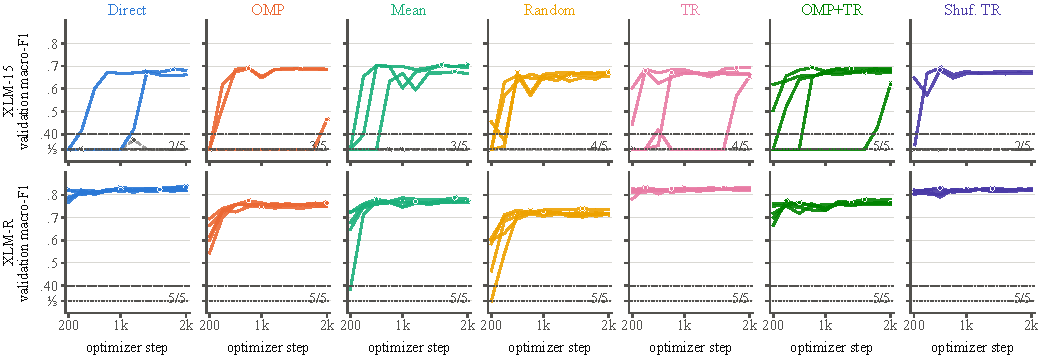
\includegraphics[width=\textwidth]{figures/fig_trajectories.pdf}
\caption{Validation \Fone{} at the ten evaluation points (steps 200–2{,}000) of all 70 runs at $n=2{,}000$, one panel per base and condition, one line per seed (\file{results/runs/*\_\_n=2000\_\_*.json}, \pfx{step\_history}). Coloured solid lines escaped; grey dashed lines never crossed the threshold. The dot marks the selected checkpoint $t^\ast$; the dotted line is the collapse basin ($1/3$), the dash-dotted line the escape threshold (0.40); the corner number is escaped/declared seeds.}
\label{fig:trajectories}
\end{figure*}

\begin{figure}[!t]
\centering
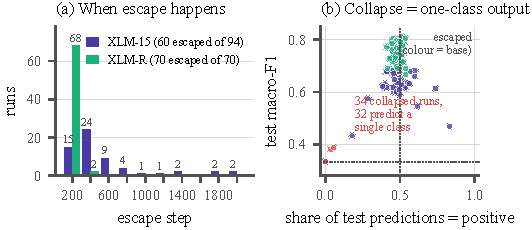
\includegraphics[width=\columnwidth]{figures/fig_escape.pdf}
\caption{Escape and collapse over all 164 runs (\file{results/runs/*.json}). (a) Step at which validation \Fone{} first exceeded 0.40 for the 130 escaped runs. (b) Share of positive predictions on the test split against test \Fone; collapsed runs (red) sit at a single-class output with \Fone{}$\approx1/3$.}
\label{fig:escape}
\end{figure}

\begin{figure*}[!t]
\centering
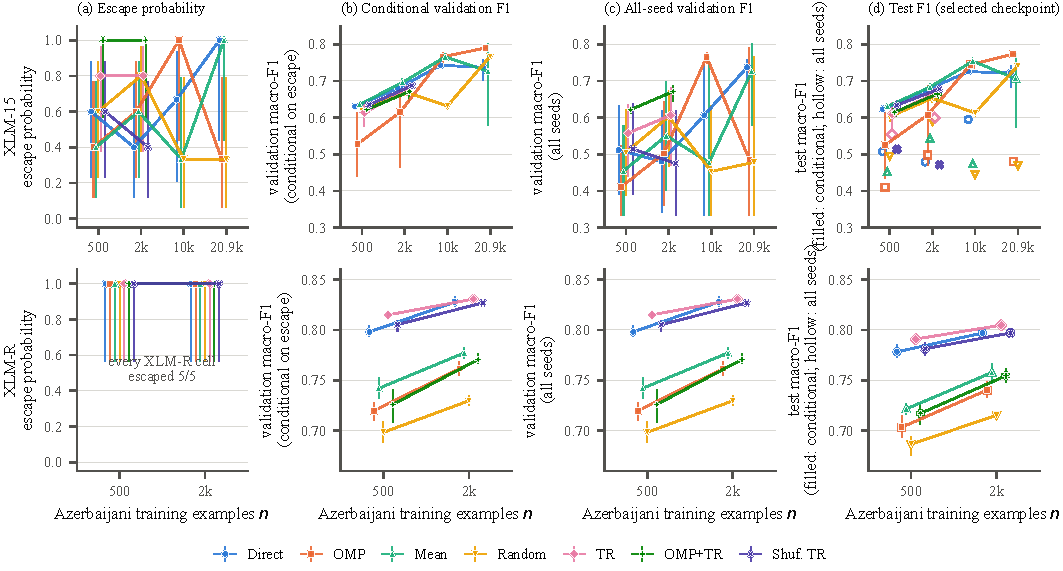
\includegraphics[width=\textwidth]{figures/fig_summary.pdf}
\caption{Failure-aware summary across Azerbaijani training sizes (top: \xlmxv; bottom: \xlmr). (a) Escape probability with Wilson 95\% intervals; every \xlmr{} cell escaped 5/5. (b) Validation \Fone{} conditional on escape and (c) over all seeds, with 10{,}000-resample percentile-bootstrap intervals (\file{results/summary.csv}). (d) Test \Fone{} at the validation-selected checkpoint, conditional (filled, with CI) and all-seed (hollow) (T1 of \file{test\_tables\_received.md}). Lines connect matched conditions and are visual guides; the size axis is a fixed-budget stress test, not a learning curve.}
\label{fig:summary}
\end{figure*}

\subsection{Direct-relative effects and multiplicity control}
\label{sec:res:effects}
Table~\ref{tab:contrastsxlmr} and Fig.~\ref{fig:forest} report every within-base contrast for \xlmr{}, where all seeds escaped and the conditional Welch family is fully measurable. Of the 86 measurable contrasts in the pre-registered family (all 42 \xlmr{} contrasts and 44 of the 54 \xlmxv{} contrasts), 27 survive Holm correction; every survivor is an \xlmr{} contrast (12 at $n=500$, 15 at $n=2{,}000$), and none involves \xlmxv, whose smallest raw Welch $p$ is 0.107. The survivors are the contrasts that separate the four donor-tokenizer arms (\OMP, \Mean, \Random, \OMPTR) from the three original-tokenizer arms (\Direct, \TR, \ShufTR)---all twelve such pairs at $n=2{,}000$ and eleven of twelve at $n=500$, where \Direct$	o$\OMPTR{} misses at Holm $p=0.063$---plus the within-transplant orderings that place \Random{} below \Mean{} at both sizes and below \OMP{} and \OMPTR{} at $n=2{,}000$. \OMP{} versus \Mean{} does not survive at either size. Every one of the six Direct-relative transplant contrasts (three initialisers at two sizes) survives, with Cohen's $d$ between $-5.3$ and $-14.9$ and bootstrap intervals excluding zero; the Holm-adjusted $p$ for \Direct$\to$\OMP{} is $7.6\times10^{-4}$ at $n=500$ and below $10^{-5}$ at $n=2{,}000$.

Turkish intermediate training is not a resolved Direct-relative improvement. \TR{} minus \Direct{} on \xlmr{} is $+0.0169$ at $n=500$ (Welch $p=0.0034$, Holm-adjusted $p=0.1955$; paired diagnostic $p=0.0021$) and $+0.0030$ at $n=2{,}000$ (Welch $p=0.372$); the corresponding test differences are $+0.0127$ and $+0.0078$. The $n=500$ direction is 5.6 times the $n=2{,}000$ direction, which is compatible with the low-resource pattern reported by Kardeş-NLU, but the current seed count does not resolve it after correction for the family it belongs to. Real versus shuffled Turkish differs by $+0.0096$ at $n=500$ (Welch $p=0.048$, Holm 1) and $+0.0038$ at $n=2{,}000$ (Welch $p=0.038$, Holm 1): the order-sensitive component (H1) is directionally positive and small, and not established. \ShufTR{} is itself indistinguishable from \Direct{} ($+0.0073$ and $-0.0008$). The interaction contrasts are informative in one direction only: \OMPTR{} is below \TR{} by $-0.0889$ and $-0.0599$ (both survive), showing that the transplant offsets the stronger original-tokenizer outcome; \OMPTR{} versus \OMP{} ($+0.0062$, $+0.0090$; Holm 1) does not show that Turkish knowledge failed or succeeded in transferring through donor rows.

\begin{table*}[!t]
\caption{Direct-relative contrasts on \xlmr{} (\file{results/stats.csv}). $\Delta$ is conditional validation \Fone{} (comparison minus \Direct) with its bootstrap 95\% CI; Welch $p$ is raw, Holm $p$ is adjusted over the 86-test family; paired $p$ is the same-seed diagnostic; $\Delta$ test is the paired test difference (T2 of \file{test\_tables\_received.md}); \checkmark{} marks family survivors.}
\label{tab:contrastsxlmr}
\centering
\footnotesize
\begin{tabular}{@{}rlrlrrrrrc@{}}
\toprule
$n$ & Contrast & $\Delta$ val & 95\% CI & Welch $p$ & Holm $p$ & Paired $p$ & $d$ & $\Delta$ test & Surv. \\
\midrule
% AUTO-GENERATED by report/ieee/tables/make_tables.py -- do not edit by hand.
% source: results/stats.csv
% source: test_tables_received.md (T2)
500 & Direct $\to$ OMP & -0.0782 & [-0.090, -0.068] & 1.0e-5 & 7.6e-4 & 3.5e-4 & -7.99 & -0.0748 & \checkmark \\
500 & Direct $\to$ Mean & -0.0560 & [-0.068, -0.044] & 1.4e-4 & 0.0090 & 0.0026 & -5.31 & -0.0566 & \checkmark \\
500 & Direct $\to$ Random & -0.0996 & [-0.112, -0.088] & 1.0e-5 & 7.6e-4 & 2.0e-4 & -9.39 & -0.0917 & \checkmark \\
500 & Direct $\to$ TR & +0.0169 & [+0.009, +0.024] & 0.0034 & 0.1955 & 0.0021 & +2.64 & +0.0127 &  \\
500 & Direct $\to$ OMP+TR & -0.0720 & [-0.092, -0.056] & 0.0011 & 0.0631 & 0.0045 & -4.43 & -0.0610 &  \\
500 & Direct $\to$ Shuf. TR & +0.0073 & [-0.001, +0.014] & 0.1386 & 1 & 0.1091 & +1.04 & +0.0031 &  \\
\midrule
2,000 & Direct $\to$ OMP & -0.0659 & [-0.075, -0.057] & $<$1e-5 & $<$1e-5 & 4.0e-5 & -8.31 & -0.0566 & \checkmark \\
2,000 & Direct $\to$ Mean & -0.0505 & [-0.058, -0.043] & $<$1e-5 & $<$1e-5 & 3.9e-4 & -7.53 & -0.0392 & \checkmark \\
2,000 & Direct $\to$ Random & -0.0980 & [-0.105, -0.091] & $<$1e-5 & $<$1e-5 & 2.0e-5 & -14.86 & -0.0816 & \checkmark \\
2,000 & Direct $\to$ TR & +0.0030 & [-0.003, +0.008] & 0.3721 & 1 & 0.3755 & +0.62 & +0.0078 &  \\
2,000 & Direct $\to$ OMP+TR & -0.0569 & [-0.064, -0.050] & $<$1e-5 & $<$1e-5 & 2.9e-4 & -8.88 & -0.0424 & \checkmark \\
2,000 & Direct $\to$ Shuf. TR & -0.0008 & [-0.006, +0.004] & 0.8026 & 1 & 0.8254 & -0.17 & +0.0001 &  \\
\bottomrule

\end{tabular}
\end{table*}

\begin{figure*}[!t]
\centering
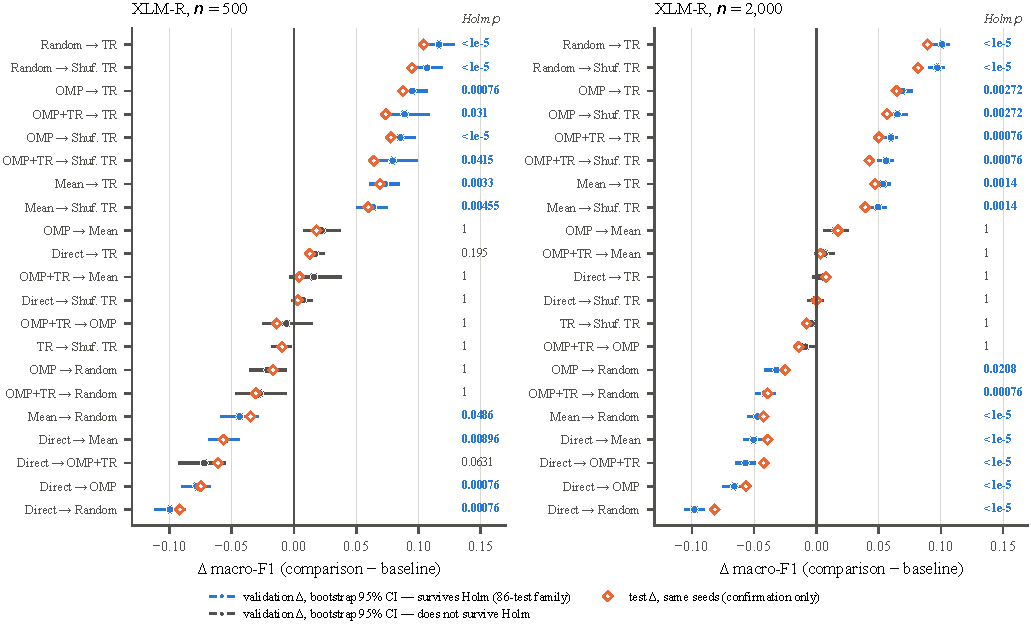
\includegraphics[width=0.95\textwidth]{figures/fig_forest.pdf}
\caption{All 42 within-base \xlmr{} contrasts (comparison minus baseline). Circles: conditional validation difference with 10{,}000-resample bootstrap 95\% CI (\file{results/stats.csv}); blue if the contrast survives Holm correction over the 86-test family, grey otherwise, with the Holm-adjusted $p$ printed at right. Hollow diamonds: paired test difference on the same five seeds (recomputed from \file{results/runs/*.json}; identical to T2/T5 of \file{test\_tables\_received.md}). Test values are confirmation only and were not used to select contrasts.}
\label{fig:forest}
\end{figure*}

\subsection{Test-side confirmation of validation-selected contrasts}
\label{sec:res:confirm}
The 27 survivors were fixed by the validation analysis and then re-tested on the held-out split with a paired $t$ over the same five seeds, Holm-corrected within the 27 (Appendix~\ref{app:survivors}). All 27 retain their sign and remain significant on test (largest within-family Holm-adjusted $p$: $1.72\times10^{-2}$, for \Mean$\to$\Random{} at $n=500$); the mean test-to-validation absolute-effect ratio is 0.874, i.e., effects shrink slightly, as expected for a checkpoint selected on validation. Across the broader set of 38 paired contrasts (both bases, any shared escaped seed), validation and test differences agree in sign for 33, and for 26 of the 27 with $|\Delta_{\mathrm{val}}|\ge0.01$; the Pearson correlation between $\Delta_{\mathrm{val}}$ and $\Delta_{\mathrm{test}}$ is 0.9898 (Fig.~\ref{fig:valtest}c). Every sign disagreement occurs where $|\Delta_{\mathrm{val}}|<0.01$ or where fewer than three seeds escaped in both arms. These calculations assess stability of the validation-selected conclusions; they do not convert the test split into a second discovery set.

\subsection{The exact sign-flip floor}
\label{sec:res:exact}
The paired $t$ statistics behind the confirmation are large (up to $|t|=61$, $p$ down to $4\times10^{-7}$) because the five seed differences are unanimous and tightly clustered. Those $p$-values rest on the normal model. Under exact sign-flip inference, Eq.~\eqref{eq:signflip}, five paired seeds admit 32 assignments and the smallest attainable two-sided $p$ is $2/32=0.0625$. All 27 survivors attain that floor on validation and on test, and all five seed differences point the same way in all 27 contrasts on both splits (Fig.~\ref{fig:signflip}): this is the maximum evidence a five-seed design can produce, and it cannot satisfy $p<0.05$ without a distributional assumption. More seeds are the only direct remedy; additional post hoc tests on the same five runs are not.

\begin{figure}[!t]
\centering
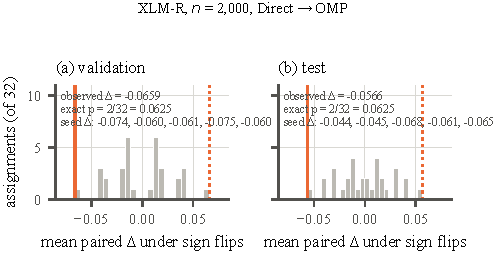
\includegraphics[width=\columnwidth]{figures/fig_signflip.pdf}
\caption{Exact sign-flip distribution for the headline contrast (\xlmr, $n=2{,}000$, \Direct$\to$\OMP), recomputed from the five per-seed differences in \file{results/runs/*.json}. The observed mean difference (solid line) and its mirror (dotted) are the two most extreme of the 32 assignments on both splits, so $p_{\mathrm{exact}}=2/32=0.0625$; the seed-level differences are printed in each panel.}
\label{fig:signflip}
\end{figure}

\subsection{Turkish source stage and degeneracy}
\label{sec:res:turkish}
Fourteen of the 30 \xlmxv{} Turkish source stages are degenerate---4 of 10 for \TR, 6 of 10 for \OMPTR, 4 of 10 for \ShufTR{} (seven at each Azerbaijani size)---with three-class Turkish \Fone{} of 0.16–0.38, i.e., the source classifier predicted one or two classes; none of the 30 \xlmr{} stages is degenerate (Turkish \Fone{} 0.69–0.79) (Fig.~\ref{fig:turkish}a). Downstream escape occurs after incompetent source stages as well as after competent ones (Fig.~\ref{fig:turkish}b), so source-stage and target-stage success are not interchangeable, and any statement that Turkish training ``stabilises'' \xlmxv{} (5/5 escapes for \OMPTR{} at both sizes) must carry the degeneracy count. Table~\ref{tab:turkish} collects the Turkish-related contrasts for both bases; on \xlmxv{} none approaches significance, and paired diagnostics are often unavailable because fewer than two seeds escaped in both arms.

\begin{figure}[!t]
\centering
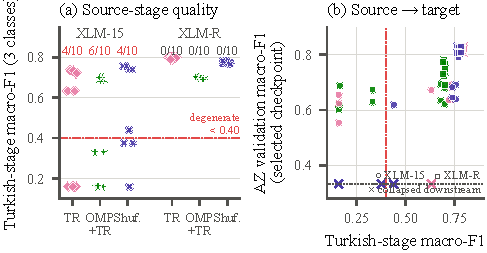
\includegraphics[width=\columnwidth]{figures/fig_turkish.pdf}
\caption{Turkish source stage (\file{results/aggregate.csv}). (a) Turkish validation \Fone{} (three classes) of every Turkish-bearing run; the count is degenerate stages per cell. (b) Downstream Azerbaijani validation \Fone{} against source-stage \Fone{} for the 60 Turkish-bearing runs; crosses are runs that collapsed downstream.}
\label{fig:turkish}
\end{figure}

\begin{table*}[!t]
\caption{Turkish-related contrasts on both bases (\file{results/stats.csv}). Escape gives escaped/declared seeds in baseline and comparison; $\Delta$ is conditional validation \Fone{} (comparison minus baseline, sign-adjusted when the stored orientation is reversed); ``shared'' is the number of seeds escaped in both arms; $\Delta$ test is the paired test difference on those seeds, recomputed from \file{results/runs/*.json}.}
\label{tab:turkish}
\centering
\footnotesize
\begin{tabular}{@{}lrlcrrrrrrrc@{}}
\toprule
Base & $n$ & Contrast & Escape & $\Delta$ cond. & Welch $p$ & Holm $p$ & Shared & Paired $p$ & $\Delta$ all-seed & $\Delta$ test & Surv. \\
\midrule
% AUTO-GENERATED by report/ieee/tables/make_tables.py -- do not edit by hand.
% source: results/stats.csv
% source: results/runs/*.json (paired test delta)
XLM-R & 500 & Direct $\to$ TR & 5/5, 5/5 & +0.0169 & 0.0034 & 0.1955 & 5 & 0.0021 & +0.0169 & +0.0127 &  \\
XLM-R & 500 & Direct $\to$ Shuf.\ TR & 5/5, 5/5 & +0.0073 & 0.1386 & 1 & 5 & 0.1091 & +0.0073 & +0.0031 &  \\
XLM-R & 500 & Shuf.\ TR $\to$ TR & 5/5, 5/5 & +0.0096 & 0.0483 & 1 & 5 & 0.0091 & +0.0096 & +0.0096 &  \\
XLM-R & 500 & Direct $\to$ OMP+TR & 5/5, 5/5 & -0.0720 & 0.0011 & 0.0631 & 5 & 0.0045 & -0.0720 & -0.0610 &  \\
XLM-R & 500 & OMP $\to$ OMP+TR & 5/5, 5/5 & +0.0062 & 0.5952 & 1 & 5 & 0.5386 & +0.0062 & +0.0138 &  \\
XLM-R & 500 & OMP+TR $\to$ TR & 5/5, 5/5 & +0.0889 & 5.0e-4 & 0.0310 & 5 & 0.0013 & +0.0889 & +0.0737 & \checkmark \\
\addlinespace[2pt]
XLM-R & 2,000 & Direct $\to$ TR & 5/5, 5/5 & +0.0030 & 0.3721 & 1 & 5 & 0.3755 & +0.0030 & +0.0078 &  \\
XLM-R & 2,000 & Direct $\to$ Shuf.\ TR & 5/5, 5/5 & -0.0008 & 0.8026 & 1 & 5 & 0.8254 & -0.0008 & +0.0001 &  \\
XLM-R & 2,000 & Shuf.\ TR $\to$ TR & 5/5, 5/5 & +0.0038 & 0.0377 & 1 & 5 & 0.0635 & +0.0038 & +0.0077 &  \\
XLM-R & 2,000 & Direct $\to$ OMP+TR & 5/5, 5/5 & -0.0569 & $<$1e-5 & $<$1e-5 & 5 & 2.9e-4 & -0.0569 & -0.0424 & \checkmark \\
XLM-R & 2,000 & OMP $\to$ OMP+TR & 5/5, 5/5 & +0.0090 & 0.1127 & 1 & 5 & 0.1756 & +0.0090 & +0.0142 &  \\
XLM-R & 2,000 & OMP+TR $\to$ TR & 5/5, 5/5 & +0.0599 & 1.0e-5 & 7.6e-4 & 5 & 2.0e-5 & +0.0599 & +0.0502 & \checkmark \\
\addlinespace[2pt]
\midrule
XLM-15 & 500 & Direct $\to$ TR & 3/5, 4/5 & -0.0165 & 0.4797 & 1 & 3 & 0.7542 & +0.0462 & +0.0070 &  \\
XLM-15 & 500 & Direct $\to$ Shuf.\ TR & 3/5, 3/5 & +0.0042 & 0.6784 & 1 & 2 & 0.5690 & +0.0025 & +0.0021 &  \\
XLM-15 & 500 & Shuf.\ TR $\to$ TR & 3/5, 4/5 & -0.0207 & 0.3939 & 1 & 2 & 0.9701 & +0.0437 & -0.0038 &  \\
XLM-15 & 500 & Direct $\to$ OMP+TR & 3/5, 5/5 & -0.0089 & 0.2924 & 1 & 3 & 0.4209 & +0.1100 & -0.0119 &  \\
XLM-15 & 500 & OMP $\to$ OMP+TR & 2/5, 5/5 & +0.0945 & 0.4728 & 1 & 2 & 0.4734 & +0.2108 & +0.0915 &  \\
XLM-15 & 500 & OMP+TR $\to$ TR & 5/5, 4/5 & -0.0076 & 0.7370 & 1 & 4 & 0.8427 & -0.0638 & -0.0039 &  \\
\addlinespace[2pt]
XLM-15 & 2,000 & Direct $\to$ TR & 2/5, 4/5 & -0.0044 & 0.6597 & 1 & 2 & 0.3488 & +0.1265 & -0.0096 &  \\
XLM-15 & 2,000 & Direct $\to$ Shuf.\ TR & 2/5, 2/5 & +0.0082 & 0.3605 & 1 & 0 & -- & -0.0049 & -- &  \\
XLM-15 & 2,000 & Shuf.\ TR $\to$ TR & 2/5, 4/5 & -0.0126 & 0.2440 & 1 & 1 & -- & +0.1315 & -0.0185 &  \\
XLM-15 & 2,000 & Direct $\to$ OMP+TR & 2/5, 5/5 & -0.0079 & 0.6001 & 1 & 2 & 0.8878 & +0.1913 & -0.0024 &  \\
XLM-15 & 2,000 & OMP $\to$ OMP+TR & 3/5, 5/5 & +0.0564 & 0.5342 & 1 & 3 & 0.4193 & +0.1689 & +0.0701 &  \\
XLM-15 & 2,000 & OMP+TR $\to$ TR & 5/5, 4/5 & +0.0035 & 0.8285 & 1 & 4 & 0.4582 & -0.0648 & -0.0079 &  \\
\addlinespace[2pt]
\bottomrule

\end{tabular}
\end{table*}

\subsection{Generalisation gap and validation–test agreement}
\label{sec:res:gap}
Across all 164 restored checkpoints the matched gap $\Delta=F_{\mathrm{test}}(t^\ast)-F_{\mathrm{val}}(t^\ast)$ has mean $-0.0126$, median $-0.0131$, standard deviation 0.0116, range $-0.0385$ to $+0.0095$, and is negative for 117 runs (Table~\ref{tab:gap}, Fig.~\ref{fig:valtest}). \xlmr{} runs have a larger gap (mean $-0.0202$, 69 of 70 negative) than \xlmxv{} runs ($-0.0069$), whose 34 collapsed runs contribute gaps near zero. A modest negative gap is the expected consequence of selecting the checkpoint on validation and supports treating the test split as confirmation rather than re-selection.

\begin{table}[!t]
\caption{Matched generalisation gap $F_{\mathrm{test}}-F_{\mathrm{val}}$ at the selected checkpoint (\file{results/aggregate.csv}).}
\label{tab:gap}
\centering
\scriptsize
\setlength{\tabcolsep}{2pt}
\begin{tabular}{@{}lrrrrrrr@{}}
\toprule
Subset & $N$ & Mean & Median & SD & Min & Max & $\Delta<0$ \\
\midrule
% AUTO-GENERATED by report/ieee/tables/make_tables.py -- do not edit by hand.
% source: results/aggregate.csv
All runs & 164 & -0.0126 & -0.0131 & 0.0116 & -0.0385 & +0.0095 & 117 \\
XLM-15 & 94 & -0.0069 & -0.0014 & 0.0101 & -0.0348 & +0.0095 & 48 \\
XLM-R & 70 & -0.0202 & -0.0202 & 0.0089 & -0.0385 & +0.0049 & 69 \\
Escaped runs & 130 & -0.0159 & -0.0163 & 0.0108 & -0.0385 & +0.0095 & 116 \\
Collapsed runs & 34 & +0.0000 & +0.0000 & 0.0018 & -0.0076 & +0.0069 & 1 \\
\bottomrule

\end{tabular}
\end{table}

\begin{figure*}[!t]
\centering
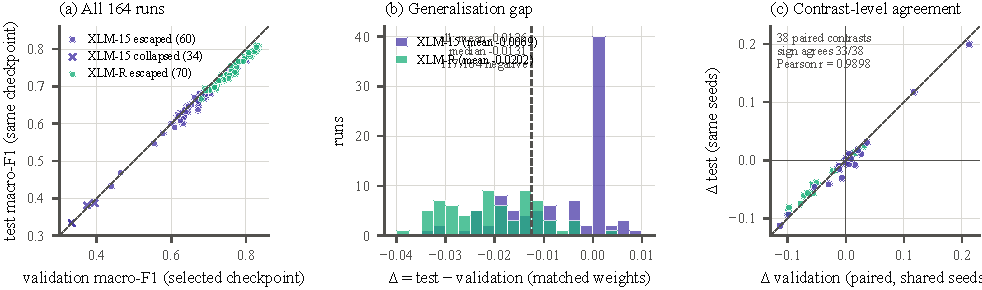
\includegraphics[width=\textwidth]{figures/fig_valtest.pdf}
\caption{Validation against test. (a) Selected-checkpoint validation \Fone{} versus test \Fone{} for all 164 runs (\file{results/aggregate.csv}). (b) Distribution of the matched gap. (c) Contrast-level agreement: paired validation difference versus paired test difference for the 38 contrasts with at least one shared escaped seed (T2 of \file{test\_tables\_received.md}).}
\label{fig:valtest}
\end{figure*}

\subsection{Fixed-step data-size sensitivity (\xlmxv)}
\label{sec:res:size}
Table~\ref{tab:size} extends the four non-Turkish \xlmxv{} conditions to $n=10{,}000$ and $n=20{,}914$ with three seeds. Escape is non-monotonic in $n$: \Direct{} escapes 3/5, 2/5, 2/3 and 3/3; \OMP{} 2/5, 3/5, 3/3 and 1/3; \Mean{} 2/5, 3/5, 1/3 and 3/3; \Random{} 3/5, 4/5, 1/3 and 1/3. At $n=20{,}914$ the single escaped \OMP{} seed reaches a conditional 0.7900 while the cell's all-seed value is 0.4856, a direct example of selection-induced ranking distortion. Because every cell receives 2{,}000 steps, exposure falls from about 125 passes to 3 across the sweep; the table is a fixed-budget robustness probe, and cells with one escaped seed have only descriptive conditional values. The only measurable higher-data contrast, \Direct$\to$\OMP{} at $n=10{,}000$ ($+0.0230$, Welch $p=0.112$), does not survive correction. H2 therefore receives no support in the form it was stated: the transplant does not help the encoder that lacks Azerbaijani pretraining, and on that encoder it is not distinguishable from its placebos.

\begin{table}[!t]
\caption{\xlmxv{} fixed-step size sensitivity (\file{results/summary.csv}, T1 of \file{test\_tables\_received.md}); five seeds at $n\le2{,}000$, three above.}
\label{tab:size}
\centering
\scriptsize
\begin{tabular}{@{}rlcrrrr@{}}
\toprule
 & & & \multicolumn{2}{c}{Validation \Fone} & \multicolumn{2}{c}{Test \Fone} \\
\cmidrule(lr){4-5}\cmidrule(lr){6-7}
$n$ & Condition & Escape & cond. & all-seed & cond. & all-seed \\
\midrule
% AUTO-GENERATED by report/ieee/tables/make_tables.py -- do not edit by hand.
% source: results/summary.csv
% source: test_tables_received.md (T1)
500 & Direct & 3/5 & 0.6306 & 0.5117 & 0.6229 & 0.5071 \\
500 & OMP & 2/5 & 0.5272 & 0.4109 & 0.5248 & 0.4100 \\
500 & Mean & 2/5 & 0.6359 & 0.4544 & 0.6302 & 0.4521 \\
500 & Random & 3/5 & 0.6192 & 0.5049 & 0.6025 & 0.4949 \\
\addlinespace[2pt]
2,000 & Direct & 2/5 & 0.6791 & 0.4799 & 0.6735 & 0.4790 \\
2,000 & OMP & 3/5 & 0.6148 & 0.5023 & 0.6076 & 0.4980 \\
2,000 & Mean & 3/5 & 0.6955 & 0.5507 & 0.6833 & 0.5434 \\
2,000 & Random & 4/5 & 0.6699 & 0.6026 & 0.6529 & 0.5890 \\
\addlinespace[2pt]
10,000 & Direct & 2/3 & 0.7427 & 0.6063 & 0.7253 & 0.5947 \\
10,000 & OMP & 3/3 & 0.7657 & 0.7657 & 0.7438 & 0.7438 \\
10,000 & Mean & 1/3 & 0.7653 & 0.4774 & 0.7539 & 0.4736 \\
10,000 & Random & 1/3 & 0.6319 & 0.4533 & 0.6129 & 0.4444 \\
\addlinespace[2pt]
20,914 & Direct & 3/3 & 0.7374 & 0.7374 & 0.7217 & 0.7217 \\
20,914 & OMP & 1/3 & 0.7900 & 0.4856 & 0.7735 & 0.4801 \\
20,914 & Mean & 3/3 & 0.7263 & 0.7263 & 0.7062 & 0.7062 \\
20,914 & Random & 1/3 & 0.7671 & 0.4780 & 0.7417 & 0.4695 \\
\bottomrule

\end{tabular}
\end{table}

\subsection{Error taxonomy on test predictions}
\label{sec:res:errors}
An automatic keyword taxonomy assigns each misclassified test example at $n=2{,}000$, pooled over both bases and all five seeds (41{,}860 predictions per condition), to one of four categories (\file{src/analysis/errors.py}), in order of precedence: false friend (the text contains a word from a Turkish–Azerbaijani false-friend list, ile{resources/false\_friends.csv}), technical vocabulary (a short list of language-reform vocabulary pairs), morphological (the example's tokens per word under the primary tokenizer exceed 4, a proxy for long suffix chains), or other (Table~\ref{tab:errors}, Fig.~\ref{fig:errors}). Error rates track the aggregate \Fone{}: 28.0\% for \TR, 29.0\% for \OMPTR, 31.5–31.6\% for \Direct, \Mean{} and \ShufTR, 33.1\% for \Random{} and 34.1\% for \OMP. The category shares are nearly identical across conditions (morphological 5.8–6.5\%, technical 1.4–1.6\%, false friend 0.2–0.3\%, other 91.8–92.3\%): the interventions change \emph{how many} errors are made, not the keyword profile of the errors. Because the taxonomy is lexical and 92\% of errors fall outside its lists, we treat it as a null result about keyword-defined error types rather than as a characterisation of the errors; a 210-row manual sample (\file{errors\_manual\_sample.csv}) was exported but not annotated within the project window.

\begin{table}[!t]
\caption{Automatic error taxonomy on test predictions at $n=2{,}000$, both bases and all seeds pooled (\file{results/errors.json}). Shares are percentages of errors.}
\label{tab:errors}
\centering
\scriptsize
\setlength{\tabcolsep}{2pt}
\begin{tabular}{@{}lrrrrrrr@{}}
\toprule
 & & & Error & \multicolumn{4}{c}{Share of errors (\%)} \\
\cmidrule(lr){5-8}
Condition & Evaluated & Errors & rate (\%) & Morph. & Techn. & False fr. & Other \\
\midrule
% AUTO-GENERATED by report/ieee/tables/make_tables.py -- do not edit by hand.
% source: results/errors.json
Direct & 41,860 & 13,176 & 31.48 & 6.5 & 1.4 & 0.2 & 91.8 \\
OMP & 41,860 & 14,286 & 34.13 & 6.0 & 1.6 & 0.3 & 92.1 \\
Mean & 41,860 & 13,221 & 31.58 & 5.9 & 1.5 & 0.3 & 92.3 \\
Random & 41,860 & 13,852 & 33.09 & 6.0 & 1.6 & 0.3 & 92.0 \\
TR & 41,860 & 11,736 & 28.04 & 6.2 & 1.5 & 0.3 & 92.0 \\
OMP+TR & 41,860 & 12,137 & 28.99 & 5.8 & 1.6 & 0.3 & 92.2 \\
Shuf. TR & 41,860 & 13,196 & 31.52 & 6.4 & 1.4 & 0.3 & 91.9 \\
\bottomrule

\end{tabular}
\end{table}

\begin{figure}[!t]
\centering
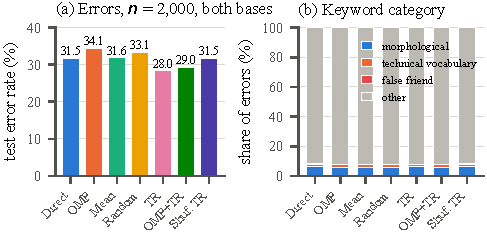
\includegraphics[width=\columnwidth]{figures/fig_errors.pdf}
\caption{Error taxonomy at $n=2{,}000$ (\file{results/errors.json}). (a) Test error rate per condition, both bases and all seeds pooled. (b) Keyword category shares; ``other'' dominates in every condition.}
\label{fig:errors}
\end{figure}

\subsection{Compute cost per condition}
\label{sec:res:cost}
Per-run wall-clock (Fig.~\ref{fig:runtime}, Table~\ref{tab:compute}) is governed by the encoder and the vocabulary: \xlmxv{} runs take 2.9–3.6 minutes and \xlmr{} runs 2.5–6.8 minutes, with the transplanted-vocabulary conditions slightly faster than the original-vocabulary ones because the tied output projection is smaller. The four data sizes differ little in wall-clock because the step budget is fixed. The whole grid consumed 8.36 process-hours on one GPU.

\section{Discussion}
\label{sec:discussion}

\subsection{What the negative transplant result establishes}
The cleanest finding is negative and implementation-bounded: the executed donor-tokenizer initialisation family damages \xlmr{} at $n=500$ and $n=2{,}000$. The conclusion triangulates across conditional and all-seed validation, restored-checkpoint test, unanimous seed direction, and three intrinsic probes (top-1 accuracy, BPC, norm calibration); bit-identical round trips and zero forward-logit deviation rule out serialisation drift. What the design cannot say is \emph{where} in the pipeline the damage originates. Functional anchors cover only 29.8\% of the donor vocabulary, so 70\% of the rows are reconstructions; the reconstruction is a 64-sparse combination of 256 cosine-nearest anchors solved in a space of a different dimension; the rows are then rescaled; the vocabulary, segmentation, truncation, tied output rows, and parameter count all change at once. Any of these could be the binding defect. Table~\ref{tab:claims} pairs each claim with its evidence and the qualifier it must carry.

Two observations narrow the space without resolving it. First, the three initialisers are ordered the same way on \xlmr{} by every measure---\Mean{} $>$ \OMP{} $>$ \Random{} on downstream \Fone; \OMP{} $>$ \Mean{} $>$ \Random{} on BPC and top-1---so the fitted solve does carry some information beyond a random placement in the anchor span, but the crude mean of the nearest anchors is at least as good downstream. That pattern is more consistent with the anchor span itself being the limiting factor than with the solver. Second, the raw OMP reconstruction inflated \xlmr{} norms by $1.91\times$ but left \xlmxv{} norms nearly unchanged ($1.13\times$), which indicates that transferring coefficients solved on unit-normalised donor rows to unnormalised base rows interacts with the base model's own norm distribution; rescaling fixes the scale but not the direction. Both observations are hypotheses for follow-up, not findings of this paper.

The result does not establish that OMP transplantation is generally harmful, that an Azerbaijani tokenizer cannot help, or that the precursor method fails on its own terms. It establishes that this implementation, on these encoders, with these anchors and this budget, does not recover the stronger original-tokenizer outcome on the encoder that already covers Azerbaijani.

\subsection{H2 and the encoder without Azerbaijani exposure}
H2 predicted that the transplant would help \xlmxv{} more than \xlmr{}. Descriptively, the cross-base difference of the \Direct$\to$\OMP{} conditional effect at $n=2{,}000$ is only 0.0017 ($-0.0643$ on \xlmxv{} vs.\ $-0.0659$ on \xlmr), and the escape-rate difference is $+0.2$ in favour of \OMP{} on \xlmxv{} (3/5 vs.\ 2/5; Fisher $p=1$). \xlmxv{}'s tokenizer deficit is real and large (3.21 tokens per word; no diacritic tokens) and the donor removes it, yet nothing downstream improves within the measurement resolution, while the intrinsic probes show the transplanted masked-LM head is as blind to Azerbaijani as the original (2 of 1{,}502 vs.\ 2 of 2{,}323). The most economical reading is that segmentation efficiency is not the binding constraint for \xlmxv{} under this budget, or that whatever the better segmentation offers is cancelled by embedding rows the encoder cannot use. The design cannot separate these, and the frequent collapse of \xlmxv{} (60/94 escapes) means that most \xlmxv{} contrasts rest on two or three surviving seeds.

\subsection{The Turkish stage: suggestive, unresolved}
\TR{} is numerically the best \xlmr{} condition at both sizes on validation and on test, its Direct-relative effect at $n=500$ is 5.6 times that at $n=2{,}000$, and the same-seed paired diagnostic at $n=500$ is small ($p=0.0021$). None of this survives correction over the family it belongs to, and the design's exact floor is 0.0625 regardless. The direction is compatible with Kardeş-NLU's low-resource claim \cite{senel2024kardes}; the magnitude, $+0.017$ \Fone{} at $n=500$, is modest. The shuffled control adds a second suggestive but unresolved layer: real Turkish beats shuffled Turkish by $+0.010$ and $+0.004$, so if there is an order-sensitive component it is smaller than the total effect, and most of the Turkish benefit, if it exists, would be attributable to shared vocabulary and extra optimisation. \ShufTR{} equals \Direct{} to within $0.01$, which means the shuffled source task on its own neither helps nor hurts measurably. On \xlmxv{}, the Turkish stage cannot be assessed at all: 14 of 30 source stages produced a classifier that predicts one or two of the three Turkish classes, so the treatment was frequently not delivered, and excluding those runs would be an outcome-based exclusion.

\subsection{Estimand choice under optimisation failure}
\xlmxv{} illustrates why a single accuracy number misleads when fine-tuning collapses. Conditional means describe selected survivors and different conditions retain different seeds; an apparently high conditional score can coincide with a poor all-seed outcome (\OMP{} at $n=20{,}914$: 0.7900 vs.\ 0.4856). Escape probability, with five seeds, cannot distinguish 2/5 from 5/5 at conventional significance. Reporting all three estimands, never pooling them, and drawing the trajectories (Fig.~\ref{fig:trajectories}) is the honest option, but a better design would predefine a joint hurdle endpoint---for example, all-seed \Fone{} with collapsed seeds charged at their score, which this paper reports but did not pre-register as primary---or would run enough seeds to estimate escape probability with useful precision. The fixed step budget, chosen to hold update opportunity constant across sizes, also means the study measures a fixed-budget regime rather than converged performance; the non-monotonic escape pattern across $n$ (Section~\ref{sec:res:size}) is a property of that regime.

\subsection{Relation to prior work}
Our tokenizer diagnostics reproduce, for Azerbaijani, the fertility gap that Rust et al.\ identified as consequential for multilingual models \cite{rust2021tokenizer}, and the Turkish–Azerbaijani overlap lift is consistent with the lexical proximity that motivates Kardeş-NLU \cite{senel2024kardes}. Unlike the embedding-initialisation literature \cite{minixhofer2022wechsel,dobler2023focus,minixhofer2024zett,goddard2025omp}, which generally reports gains for the language whose tokenizer is installed, we observe a loss on the encoder that already covered the language and no gain on the encoder that did not, under a training-free initialisation and a short fine-tuning budget. The most plausible reconciliation is that those methods are usually followed by continued pretraining or larger adaptation budgets, which our protocol deliberately excluded to isolate the initialisation itself; our result is therefore about the initialisation, not about tokenizer adaptation with further training. The seed instability we document is in line with the fine-tuning-stability literature \cite{dodge2020finetuning,mosbach2021stability}, and our use of an explicit family, Holm correction, and an exact floor follows the recommendations of Dror et al.\ \cite{dror2018hitchhiker} and Bouthillier et al.\ \cite{bouthillier2021variance}.

\begin{table*}[!t]
\caption{Claim–evidence map. Every headline claim, the artefact that backs it, and the qualifier that must accompany it wherever the claim is repeated.}
\label{tab:claims}
\centering
\footnotesize
\begin{tabular}{@{}L{5.0cm}L{5.2cm}L{6.3cm}@{}}
\toprule
Claim & Evidence (table / figure; file) & Mandatory qualifier \\
\midrule
The implemented OMP transplant lowers \xlmr{} \Fone{} at $n\in\{500,2000\}$ & Tables~\ref{tab:results2000}, \ref{tab:results500}, \ref{tab:contrastsxlmr}; Fig.~\ref{fig:forest}; \file{stats.csv}, T5 & Implementation-bounded; compound intervention; parametric survivor; exact floor 0.0625 \\
Intrinsic probes corroborate the \xlmr{} failure & Table~\ref{tab:intrinsic}; Fig.~\ref{fig:intrinsic}; \file{controls\_\_*.json} & Diagnostics on 300 training lines; masked positions differ between tokenizers \\
Placebos order \Mean{} $>$ \OMP{} $>$ \Random{} downstream on \xlmr & Table~\ref{tab:contrastsxlmr}; Fig.~\ref{fig:forest} & \OMP$\to$\Mean{} does not survive Holm; \Random{} contrasts do \\
Turkish stage is numerically best on \xlmr & Tables~\ref{tab:results2000}, \ref{tab:results500}, \ref{tab:turkish} & Direct-relative gain does not survive Holm (0.1955 at $n=500$); real-vs-shuffled unresolved \\
27 of 86 contrasts survive Holm, all on \xlmr; 27/27 confirmed on test & Table~\ref{tab:survivors} (Appendix); T5, T6 & Model-based; exact sign-flip floor 0.0625 with five seeds \\
\xlmxv{} is dominated by collapse & Figs.~\ref{fig:trajectories}, \ref{fig:escape}, \ref{fig:summary}; \file{aggregate.csv} & 60/94 escapes; conditional and all-seed estimands diverge; no \xlmxv{} contrast survives \\
14 of 30 \xlmxv{} Turkish stages degenerate & Fig.~\ref{fig:turkish}; Table~\ref{tab:turkish} & Reported, not excluded; treatment often not delivered \\
Transplant removes the \xlmxv{} segmentation deficit & Table~\ref{tab:tokenizer}; Fig.~\ref{fig:tokenizer} & Efficiency does not imply usable embeddings (H2 unsupported) \\
Test confirms validation (gap $-0.0126$; $r=0.9898$) & Table~\ref{tab:gap}; Fig.~\ref{fig:valtest} & Confirmation only; test never used for selection \\
Grid fits the compute envelope & Table~\ref{tab:compute}; Fig.~\ref{fig:runtime} & 8.36 process-h on a rented H100; peak memory \NM \\
\bottomrule
\end{tabular}
\end{table*}

\section{Limitations and Threats to Validity}
\label{sec:limitations}

\paragraph{Construct validity} Tokenizer replacement jointly changes segmentation, vocabulary, embedding rows, tied output rows, truncation (1.257\%$\to$0.351\% of examples for \xlmxv), and parameter count. Word shuffling changes order, fluency, and source-task difficulty. Neither contrast isolates a single linguistic mechanism; Table~\ref{tab:identification} is the binding statement of what is identified. Five of the twelve (tokenizer, pre-stage) combinations---the placebos with a Turkish stage and the donor tokenizer with shuffled Turkish---were not run, so the interaction between transplant quality and the Turkish stage is observed only for OMP.

\paragraph{Model confounding} The bases differ in architecture, pretraining coverage, tokenizer scheme, and non-embedding capacity ($1.8\times$). Cross-base differences cannot be attributed to Azerbaijani pretraining exposure alone, and the two encoders were not matched on any of these axes.

\paragraph{Optimisation validity} All cells receive the same 2{,}000-step budget despite dataset sizes spanning $42\times$, so the size sweep measures a fixed-budget regime. \xlmxv{} collapses in 34 of 94 runs, 14 of its 30 Turkish source stages are degenerate, and several conditional cells contain one or two observations. The experiment does not measure converged performance, and it does not measure tokenizer adaptation followed by continued pretraining.

\paragraph{Statistical validity} Only five (or three) seeds exist before escape conditioning. Exact paired inference cannot cross $p=0.05$ with five seeds; every significance statement is model-based. Max-validation checkpoint selection and validation reporting use the same observations, which is why the test split is reported and why its gap is negative. Escape-rate contrasts have no power at this seed count. Holm control is applied to the pre-registered Welch family only; the paired, all-seed, and Fisher analyses are diagnostics.

\paragraph{Data and label validity} The upstream Azerbaijani revision is unpinned; the archived \file{data.tgz} is the only exact copy and the manifests are the only proof of identity. Pre-grid and grid splits differ by one example, so the human audit characterises the dataset, not the holdout. Unconditioned retained-label agreement is 65.67\%, and the two annotators differ by nine points against gold; a non-trivial share of test labels is therefore uncertain, which bounds attainable \Fone{} and adds noise common to all conditions. Both datasets are user-generated sentiment text; the study does not speak to other domains or to formal Azerbaijani.

\paragraph{Test-protocol validity} The 164-entry ledger shows one test evaluation per run, at the verified restored checkpoint. Test-side inference is confirmation of validation-selected survivors, not discovery, and its paired tests inherit the five-seed exact floor.

\paragraph{Reproducibility and resources} The original lock did not describe the executed stack; two dependencies were undeclared; per-run weights and the Turkish cache are not distributed; peak GPU memory during the grid is \NM; the grid ran on a rented H100 rather than the course workstation, in one stream. A clean-checkout reproduction on the course machine was not performed within the project window.

\paragraph{External validity} Evidence is limited to one binary sentiment dataset, one Turkish source task, one donor tokenizer, one sparse-reconstruction configuration ($k=64$, $m=256$, functional anchors), and two unmatched encoders. It does not establish transfer to other tasks, Azerbaijani varieties, donors, or architectures, and $k$ and $m$ were not ablated.

\paragraph{Licensing} LocalDoc is CC-BY-NC-SA-4.0, \xlmxv{} is CC-BY-NC-4.0, the HPLT donor is Apache-2.0, \xlmr{} is MIT, and the captured TRSAv1 card declares no licence. Redistribution rights must be checked per artefact; the non-commercial terms bind any downstream use of the dataset and of \xlmxv{}-derived checkpoints.

\section{Conclusion and Future Work}
\label{sec:conclusion}
Under a pre-registered, fixed-budget protocol with 164 completed runs, the implemented OMP tokenizer-transplant pipeline consistently harms \xlmr{} at low and reference Azerbaijani data sizes---by $0.05$–$0.10$ \Fone{} on validation and on the restored-checkpoint test split, in every seed, and with the ordering \Mean{} $>$ \OMP{} $>$ \Random{} among initialisers---while its intrinsic probes show that the reconstructed embedding rows do not preserve what the encoder's masked-LM head needs. On \xlmxv{}, which lacks Azerbaijani pretraining and has a severe segmentation deficit that the donor removes, the transplant produces no measurable improvement and is entangled with frequent optimisation collapse. Turkish intermediate training is directionally favourable for \xlmr{}, more so at $n=500$, but is not statistically resolved against direct fine-tuning after correction over the primary family, and its order-sensitive component, if any, is smaller than its total effect. Twenty-seven contrasts survive Holm correction, all on \xlmr{}, and all twenty-seven keep their sign and significance on test; with five seeds, none can exceed the exact sign-flip floor of $0.0625$.

The defensible contribution is a transparent comparison of adaptation pipelines with explicit failure-aware estimands, restored-checkpoint testing, multiplicity control, intrinsic diagnostics, source-stage accounting, and artefact-level disclosure of data provenance, software, compute, and test-set usage. The experiment does not show that Turkish transfer is ineffective, that an Azerbaijani tokenizer cannot help, that OMP transplantation is generally harmful, or that syntax has been isolated.

A stronger follow-up requires, in order of value: more independent seeds (the only remedy for the exact floor and for escape-rate power); a pre-registered joint hurdle endpoint combining failure probability and quality; an ablation of the anchor mode, $k$, $m$, and the norm-rescaling step, with an independently validated reference implementation of the transplant; a continued-pretraining arm after transplantation to separate initialisation from adaptation; gated or repeated Turkish source stages so that the treatment is always delivered; the five omitted (tokenizer, pre-stage) combinations; pinned data revisions and a clean-checkout reproduction on the course workstation with measured peak memory; and retention of selected checkpoints and predictions for error analysis beyond keyword taxonomies.

\section*{Tools and Acknowledgements}
We thank AI Academy and the National Artificial Intelligence Center for the course context and the DLE-AI-202 brief that shaped the compute and reporting requirements. Emil Jafarov originated the project idea and was the main contributor; authors are listed alphabetically by surname. Correspondence: \pfx{emil.jafarov.II@aiacademy.az}.

\paragraph{AI-assistance disclosure} Large language models were used substantially in this project: for drafting and editing the paper text, for inspecting result artefacts and checking the consistency of numbers against files, for converting tables, for writing and debugging the analysis, figure, and table scripts in \file{report/ieee/}, and for parts of the experiment code and its documentation. They did not generate experimental observations, alter result files, or train models. Every number in this paper was recomputed from the committed result files by the scripts named in the captions, and every claim, figure, and line of code is understood by and defensible by the authors. The experiments themselves ran with PyTorch \cite{paszke2019pytorch}, Transformers \cite{wolf2020transformers}, scikit-learn \cite{pedregosa2011sklearn}, and the Hugging Face model and dataset hubs.


\bibliographystyle{IEEEtran}
\bibliography{refs}

\appendices

\section{Complete 36-Cell Results}
\label{app:cells}
Table~\ref{tab:allcells} lists every cell of the grid with escape rate and Wilson interval, conditional and all-seed validation \Fone{} with bootstrap intervals, test \Fone{} at the restored selected checkpoint, the number of seeds that escaped mid-training but ended collapsed, and the number of degenerate Turkish source stages.

\begin{table*}[!t]
\caption{All 36 cells (\file{results/summary.csv}; test columns from T1 of \file{evidence/supplemental/test\_tables\_received.md}; both exact aggregates of \file{results/runs/*.json}). Wilson and bootstrap intervals are 95\%; ``E$\to$C'' is escaped-then-terminal-collapsed seeds; ``TR deg.'' is degenerate Turkish source stages (-- for conditions without a Turkish stage).}
\label{tab:allcells}
\centering
\scriptsize
\setlength{\tabcolsep}{3pt}
\begin{tabular}{@{}lrlclrlrlrlrcc@{}}
\toprule
 & & & \multicolumn{2}{c}{Escape} & \multicolumn{2}{c}{Val.\ cond.} & \multicolumn{2}{c}{Val.\ all-seed} & \multicolumn{2}{c}{Test cond.} & Test & & TR \\
\cmidrule(lr){4-5}\cmidrule(lr){6-7}\cmidrule(lr){8-9}\cmidrule(lr){10-11}
Base & $n$ & Condition & rate & Wilson & \Fone & CI & \Fone & CI & \Fone & CI & all-seed & E$\to$C & deg. \\
\midrule
% AUTO-GENERATED by report/ieee/tables/make_tables.py -- do not edit by hand.
% source: results/summary.csv
% source: test_tables_received.md (T1)
XLM-15 & 500 & Direct & 3/5 & [0.23, 0.88] & 0.6306 & [0.621, 0.639] & 0.5117 & [0.391, 0.632] & 0.6229 & [0.618, 0.632] & 0.5071 & 0 & 0 \\
XLM-15 & 500 & OMP & 2/5 & [0.12, 0.77] & 0.5272 & [0.440, 0.614] & 0.4109 & [0.333, 0.523] & 0.5248 & [0.433, 0.617] & 0.4100 & 1 & 0 \\
XLM-15 & 500 & Mean & 2/5 & [0.12, 0.77] & 0.6359 & [0.627, 0.645] & 0.4544 & [0.333, 0.579] & 0.6302 & [0.629, 0.631] & 0.4521 & 0 & 0 \\
XLM-15 & 500 & Random & 3/5 & [0.23, 0.88] & 0.6192 & [0.609, 0.632] & 0.5049 & [0.389, 0.621] & 0.6025 & [0.590, 0.618] & 0.4949 & 0 & 0 \\
XLM-15 & 500 & TR & 4/5 & [0.38, 0.96] & 0.6141 & [0.575, 0.639] & 0.5580 & [0.439, 0.635] & 0.6090 & [0.569, 0.641] & 0.5539 & 0 & 2 \\
XLM-15 & 500 & OMP+TR & 5/5 & [0.57, 1.00] & 0.6217 & [0.611, 0.630] & 0.6217 & [0.611, 0.630] & 0.6142 & [0.607, 0.619] & 0.6142 & 0 & 3 \\
XLM-15 & 500 & Shuf. TR & 3/5 & [0.23, 0.88] & 0.6348 & [0.620, 0.646] & 0.5143 & [0.391, 0.638] & 0.6336 & [0.622, 0.647] & 0.5135 & 0 & 2 \\
\addlinespace[2pt]
XLM-15 & 2,000 & Direct & 2/5 & [0.12, 0.77] & 0.6791 & [0.674, 0.684] & 0.4799 & [0.342, 0.618] & 0.6735 & [0.671, 0.676] & 0.4790 & 0 & 0 \\
XLM-15 & 2,000 & OMP & 3/5 & [0.23, 0.88] & 0.6148 & [0.464, 0.691] & 0.5023 & [0.360, 0.645] & 0.6076 & [0.468, 0.687] & 0.4980 & 0 & 0 \\
XLM-15 & 2,000 & Mean & 3/5 & [0.23, 0.88] & 0.6955 & [0.675, 0.706] & 0.5507 & [0.402, 0.700] & 0.6833 & [0.681, 0.687] & 0.5434 & 0 & 0 \\
XLM-15 & 2,000 & Random & 4/5 & [0.38, 0.96] & 0.6699 & [0.664, 0.673] & 0.6026 & [0.467, 0.673] & 0.6529 & [0.641, 0.666] & 0.5890 & 0 & 0 \\
XLM-15 & 2,000 & TR & 4/5 & [0.38, 0.96] & 0.6747 & [0.661, 0.687] & 0.6064 & [0.469, 0.683] & 0.6663 & [0.656, 0.677] & 0.5997 & 0 & 2 \\
XLM-15 & 2,000 & OMP+TR & 5/5 & [0.57, 1.00] & 0.6712 & [0.645, 0.689] & 0.6712 & [0.645, 0.689] & 0.6645 & [0.644, 0.679] & 0.6645 & 0 & 3 \\
XLM-15 & 2,000 & Shuf. TR & 2/5 & [0.12, 0.77] & 0.6873 & [0.682, 0.692] & 0.4750 & [0.333, 0.618] & 0.6784 & [0.678, 0.679] & 0.4714 & 0 & 2 \\
\addlinespace[2pt]
XLM-15 & 10,000 & Direct & 2/3 & [0.21, 0.94] & 0.7427 & [0.740, 0.746] & 0.6063 & [0.333, 0.746] & 0.7253 & [0.724, 0.727] & 0.5947 & 0 & 0 \\
XLM-15 & 10,000 & OMP & 3/3 & [0.44, 1.00] & 0.7657 & [0.749, 0.778] & 0.7657 & [0.749, 0.778] & 0.7438 & [0.730, 0.754] & 0.7438 & 0 & 0 \\
XLM-15 & 10,000 & Mean & 1/3 & [0.06, 0.79] & 0.7653 & [0.765, 0.765] & 0.4774 & [0.333, 0.765] & 0.7539 & [0.754, 0.754] & 0.4736 & 0 & 0 \\
XLM-15 & 10,000 & Random & 1/3 & [0.06, 0.79] & 0.6319 & [0.632, 0.632] & 0.4533 & [0.333, 0.632] & 0.6129 & [0.613, 0.613] & 0.4444 & 0 & 0 \\
\addlinespace[2pt]
XLM-15 & 20,914 & Direct & 3/3 & [0.44, 1.00] & 0.7374 & [0.701, 0.758] & 0.7374 & [0.701, 0.758] & 0.7217 & [0.682, 0.743] & 0.7217 & 0 & 0 \\
XLM-15 & 20,914 & OMP & 1/3 & [0.06, 0.79] & 0.7900 & [0.790, 0.790] & 0.4856 & [0.333, 0.790] & 0.7735 & [0.773, 0.773] & 0.4801 & 0 & 0 \\
XLM-15 & 20,914 & Mean & 3/3 & [0.44, 1.00] & 0.7263 & [0.578, 0.801] & 0.7263 & [0.578, 0.801] & 0.7062 & [0.574, 0.775] & 0.7062 & 1 & 0 \\
XLM-15 & 20,914 & Random & 1/3 & [0.06, 0.79] & 0.7671 & [0.767, 0.767] & 0.4780 & [0.333, 0.767] & 0.7417 & [0.742, 0.742] & 0.4695 & 0 & 0 \\
\addlinespace[2pt]
\midrule
XLM-R & 500 & Direct & 5/5 & [0.57, 1.00] & 0.7980 & [0.794, 0.804] & 0.7980 & [0.794, 0.804] & 0.7783 & [0.773, 0.785] & 0.7783 & 0 & 0 \\
XLM-R & 500 & OMP & 5/5 & [0.57, 1.00] & 0.7198 & [0.710, 0.728] & 0.7198 & [0.710, 0.728] & 0.7035 & [0.693, 0.715] & 0.7035 & 0 & 0 \\
XLM-R & 500 & Mean & 5/5 & [0.57, 1.00] & 0.7421 & [0.732, 0.752] & 0.7421 & [0.732, 0.752] & 0.7217 & [0.716, 0.727] & 0.7217 & 0 & 0 \\
XLM-R & 500 & Random & 5/5 & [0.57, 1.00] & 0.6985 & [0.688, 0.709] & 0.6985 & [0.688, 0.709] & 0.6867 & [0.676, 0.694] & 0.6867 & 0 & 0 \\
XLM-R & 500 & TR & 5/5 & [0.57, 1.00] & 0.8149 & [0.810, 0.819] & 0.8149 & [0.810, 0.819] & 0.7910 & [0.788, 0.794] & 0.7910 & 0 & 0 \\
XLM-R & 500 & OMP+TR & 5/5 & [0.57, 1.00] & 0.7261 & [0.708, 0.741] & 0.7261 & [0.708, 0.741] & 0.7173 & [0.706, 0.727] & 0.7173 & 0 & 0 \\
XLM-R & 500 & Shuf. TR & 5/5 & [0.57, 1.00] & 0.8054 & [0.799, 0.810] & 0.8054 & [0.799, 0.810] & 0.7814 & [0.774, 0.787] & 0.7814 & 0 & 0 \\
\addlinespace[2pt]
XLM-R & 2,000 & Direct & 5/5 & [0.57, 1.00] & 0.8277 & [0.823, 0.833] & 0.8277 & [0.823, 0.833] & 0.7970 & [0.793, 0.801] & 0.7970 & 0 & 0 \\
XLM-R & 2,000 & OMP & 5/5 & [0.57, 1.00] & 0.7618 & [0.755, 0.769] & 0.7618 & [0.755, 0.769] & 0.7404 & [0.733, 0.749] & 0.7404 & 0 & 0 \\
XLM-R & 2,000 & Mean & 5/5 & [0.57, 1.00] & 0.7772 & [0.772, 0.783] & 0.7772 & [0.772, 0.783] & 0.7578 & [0.747, 0.767] & 0.7578 & 0 & 0 \\
XLM-R & 2,000 & Random & 5/5 & [0.57, 1.00] & 0.7297 & [0.725, 0.735] & 0.7297 & [0.725, 0.735] & 0.7154 & [0.714, 0.717] & 0.7154 & 0 & 0 \\
XLM-R & 2,000 & TR & 5/5 & [0.57, 1.00] & 0.8307 & [0.829, 0.832] & 0.8307 & [0.829, 0.832] & 0.8048 & [0.803, 0.808] & 0.8048 & 0 & 0 \\
XLM-R & 2,000 & OMP+TR & 5/5 & [0.57, 1.00] & 0.7708 & [0.766, 0.776] & 0.7708 & [0.766, 0.776] & 0.7546 & [0.748, 0.762] & 0.7546 & 0 & 0 \\
XLM-R & 2,000 & Shuf. TR & 5/5 & [0.57, 1.00] & 0.8269 & [0.825, 0.829] & 0.8269 & [0.825, 0.829] & 0.7971 & [0.795, 0.801] & 0.7971 & 0 & 0 \\
\addlinespace[2pt]
\addlinespace[2pt]
\addlinespace[2pt]
\bottomrule

\end{tabular}
\end{table*}

\section{The 27 Holm-Surviving Contrasts and Their Test Confirmation}
\label{app:survivors}
Table~\ref{tab:survivors} lists the contrasts that survive Holm correction over the 86-test validation family, with the paired $t$ test on test \Fone{} over the same five seeds and the Holm adjustment within the 27. All 27 are \xlmr{} contrasts; every seed difference has the same sign on both splits; the exact sign-flip $p$ is $0.0625$ for every row on both splits; mean shrinkage $|\Delta_{\mathrm{test}}|/|\Delta_{\mathrm{val}}|$ is 0.874.

\begin{table}[!t]
\caption{Validation survivors and test confirmation (T5 of \file{evidence/supplemental/test\_tables\_received.md}; \file{results/stats.csv}).}
\label{tab:survivors}
\centering
\scriptsize
\setlength{\tabcolsep}{1.4pt}
\begin{tabular}{@{}rlrrrrr@{}}
\toprule
$n$ & Contrast & $\Delta$ val & $\Delta$ test & $t$ (test) & $p$ (test) & Holm/27 \\
\midrule
% AUTO-GENERATED by report/ieee/tables/make_tables.py -- do not edit by hand.
% source: evidence/supplemental/test_tables_received.md (T5)
% source: results/stats.csv
500 & Direct $\to$ OMP & -0.0782 & -0.0748 & -10.71 & 4.30e-04 & 5.20e-03 \\
500 & Direct $\to$ Mean & -0.0560 & -0.0566 & -8.84 & 9.04e-04 & 8.54e-03 \\
500 & Direct $\to$ Random & -0.0996 & -0.0917 & -15.65 & 9.73e-05 & 2.04e-03 \\
500 & OMP+TR $\to$ TR & +0.0889 & +0.0737 & +10.47 & 4.70e-04 & 5.20e-03 \\
500 & OMP+TR $\to$ Shuf. TR & +0.0793 & +0.0641 & +8.97 & 8.54e-04 & 8.54e-03 \\
500 & OMP $\to$ TR & +0.0951 & +0.0875 & +12.26 & 2.54e-04 & 4.83e-03 \\
500 & OMP $\to$ Shuf. TR & +0.0855 & +0.0779 & +11.42 & 3.36e-04 & 5.07e-03 \\
500 & Mean $\to$ Random & -0.0436 & -0.0350 & -4.81 & 8.59e-03 & 1.72e-02 \\
500 & Mean $\to$ TR & +0.0729 & +0.0693 & +17.20 & 6.70e-05 & 1.61e-03 \\
500 & Mean $\to$ Shuf. TR & +0.0633 & +0.0597 & +13.56 & 1.71e-04 & 3.43e-03 \\
500 & Random $\to$ TR & +0.1165 & +0.1043 & +16.16 & 8.58e-05 & 1.89e-03 \\
500 & Random $\to$ Shuf. TR & +0.1069 & +0.0947 & +12.01 & 2.76e-04 & 4.96e-03 \\
2,000 & Direct $\to$ OMP+TR & -0.0569 & -0.0424 & -7.31 & 1.86e-03 & 1.08e-02 \\
2,000 & Direct $\to$ OMP & -0.0659 & -0.0566 & -10.92 & 4.00e-04 & 5.20e-03 \\
2,000 & Direct $\to$ Mean & -0.0505 & -0.0392 & -7.20 & 1.97e-03 & 1.08e-02 \\
2,000 & Direct $\to$ Random & -0.0980 & -0.0816 & -36.97 & 3.20e-06 & 8.31e-05 \\
2,000 & OMP+TR $\to$ Random & -0.0411 & -0.0392 & -8.09 & 1.27e-03 & 9.53e-03 \\
2,000 & OMP+TR $\to$ TR & +0.0599 & +0.0502 & +11.15 & 3.68e-04 & 5.15e-03 \\
2,000 & OMP+TR $\to$ Shuf. TR & +0.0561 & +0.0425 & +11.95 & 2.81e-04 & 4.96e-03 \\
2,000 & OMP $\to$ Random & -0.0320 & -0.0250 & -4.65 & 9.64e-03 & 1.72e-02 \\
2,000 & OMP $\to$ TR & +0.0690 & +0.0644 & +11.59 & 3.17e-04 & 5.07e-03 \\
2,000 & OMP $\to$ Shuf. TR & +0.0651 & +0.0567 & +17.02 & 6.99e-05 & 1.61e-03 \\
2,000 & Mean $\to$ Random & -0.0475 & -0.0424 & -6.93 & 2.28e-03 & 1.08e-02 \\
2,000 & Mean $\to$ TR & +0.0535 & +0.0470 & +8.22 & 1.19e-03 & 9.53e-03 \\
2,000 & Mean $\to$ Shuf. TR & +0.0496 & +0.0393 & +7.38 & 1.80e-03 & 1.08e-02 \\
2,000 & Random $\to$ TR & +0.1010 & +0.0894 & +61.23 & 4.26e-07 & 1.15e-05 \\
2,000 & Random $\to$ Shuf. TR & +0.0972 & +0.0817 & +34.30 & 4.31e-06 & 1.08e-04 \\
\bottomrule

\end{tabular}
\end{table}

\section{All Paired Contrasts}
\label{app:paired}
Table~\ref{tab:pairedall} reports the paired validation and test differences on seeds that escaped in both arms for the 42 key contrasts of the companion table (38 with at least one shared seed), together with the all-seed differences, for both bases.

\begin{table*}[!t]
\caption{Paired and all-seed contrasts, both bases (T2 of \file{evidence/supplemental/test\_tables\_received.md}). ``n/a'': no seed escaped in both arms.}
\label{tab:pairedall}
\centering
\scriptsize
\setlength{\tabcolsep}{4pt}
\begin{tabular}{@{}lrlrrrcrr@{}}
\toprule
Base & $n$ & Contrast & $\Delta$ val (paired) & $\Delta$ test (paired) & Shared & Same sign & $\Delta$ val (all-seed) & $\Delta$ test (all-seed) \\
\midrule
% AUTO-GENERATED by report/ieee/tables/make_tables.py -- do not edit by hand.
% source: evidence/supplemental/test_tables_received.md (T2)
XLM-R & 500 & Direct $\to$ TR & +0.0169 & +0.0127 & 5 & yes & +0.0169 & +0.0127 \\
XLM-R & 500 & Direct $\to$ OMP+TR & -0.0720 & -0.0610 & 5 & yes & -0.0720 & -0.0610 \\
XLM-R & 500 & Direct $\to$ Shuf. TR & +0.0073 & +0.0031 & 5 & yes & +0.0073 & +0.0031 \\
XLM-R & 500 & Direct $\to$ OMP & -0.0782 & -0.0748 & 5 & yes & -0.0782 & -0.0748 \\
XLM-R & 500 & Direct $\to$ Mean & -0.0560 & -0.0566 & 5 & yes & -0.0560 & -0.0566 \\
XLM-R & 500 & Direct $\to$ Random & -0.0996 & -0.0917 & 5 & yes & -0.0996 & -0.0917 \\
XLM-R & 500 & Random $\to$ OMP & +0.0213 & +0.0168 & 5 & yes & +0.0213 & +0.0168 \\
XLM-R & 500 & Mean $\to$ OMP & -0.0223 & -0.0182 & 5 & yes & -0.0223 & -0.0182 \\
XLM-R & 2,000 & Direct $\to$ TR & +0.0030 & +0.0078 & 5 & yes & +0.0030 & +0.0078 \\
XLM-R & 2,000 & Direct $\to$ OMP+TR & -0.0569 & -0.0424 & 5 & yes & -0.0569 & -0.0424 \\
XLM-R & 2,000 & Direct $\to$ Shuf. TR & -0.0008 & +0.0001 & 5 & NO & -0.0008 & +0.0001 \\
XLM-R & 2,000 & Direct $\to$ OMP & -0.0659 & -0.0566 & 5 & yes & -0.0659 & -0.0566 \\
XLM-R & 2,000 & Direct $\to$ Mean & -0.0505 & -0.0392 & 5 & yes & -0.0505 & -0.0392 \\
XLM-R & 2,000 & Direct $\to$ Random & -0.0980 & -0.0816 & 5 & yes & -0.0980 & -0.0816 \\
XLM-R & 2,000 & Random $\to$ OMP & +0.0320 & +0.0250 & 5 & yes & +0.0320 & +0.0250 \\
XLM-R & 2,000 & Mean $\to$ OMP & -0.0155 & -0.0174 & 5 & yes & -0.0155 & -0.0174 \\
XLM-15 & 500 & Direct $\to$ TR & +0.0033 & +0.0070 & 3 & yes & +0.0462 & +0.0468 \\
XLM-15 & 500 & Direct $\to$ OMP+TR & -0.0124 & -0.0119 & 3 & yes & +0.1100 & +0.1071 \\
XLM-15 & 500 & Direct $\to$ Shuf. TR & -0.0008 & +0.0021 & 2 & NO & +0.0025 & +0.0064 \\
XLM-15 & 500 & Direct $\to$ OMP & -0.0991 & -0.0937 & 2 & yes & -0.1008 & -0.0971 \\
XLM-15 & 500 & Direct $\to$ Mean & +0.0056 & +0.0113 & 1 & yes & -0.0573 & -0.0550 \\
XLM-15 & 500 & Direct $\to$ Random & -0.0297 & -0.0418 & 1 & yes & -0.0068 & -0.0122 \\
XLM-15 & 500 & Random $\to$ OMP & n/a & n/a & 0 & -- & -0.0940 & -0.0849 \\
XLM-15 & 500 & Mean $\to$ OMP & -0.0128 & -0.0120 & 1 & yes & -0.0435 & -0.0422 \\
XLM-15 & 2,000 & Direct $\to$ TR & -0.0119 & -0.0096 & 2 & yes & +0.1265 & +0.1207 \\
XLM-15 & 2,000 & Direct $\to$ OMP+TR & +0.0022 & -0.0024 & 2 & NO & +0.1913 & +0.1855 \\
XLM-15 & 2,000 & Direct $\to$ Shuf. TR & n/a & n/a & 0 & -- & -0.0049 & -0.0076 \\
XLM-15 & 2,000 & Direct $\to$ OMP & +0.0156 & -0.0082 & 1 & NO & +0.0224 & +0.0189 \\
XLM-15 & 2,000 & Direct $\to$ Mean & +0.0264 & +0.0106 & 2 & yes & +0.0708 & +0.0643 \\
XLM-15 & 2,000 & Direct $\to$ Random & -0.0067 & -0.0305 & 2 & yes & +0.1227 & +0.1099 \\
XLM-15 & 2,000 & Random $\to$ OMP & -0.0539 & -0.0465 & 3 & yes & -0.1003 & -0.0910 \\
XLM-15 & 2,000 & Mean $\to$ OMP & -0.0001 & -0.0043 & 2 & yes & -0.0484 & -0.0454 \\
XLM-15 & 10,000 & Direct $\to$ OMP & +0.0206 & +0.0170 & 2 & yes & +0.1594 & +0.1492 \\
XLM-15 & 10,000 & Direct $\to$ Mean & n/a & n/a & 0 & -- & -0.1289 & -0.1211 \\
XLM-15 & 10,000 & Direct $\to$ Random & -0.1137 & -0.1136 & 1 & yes & -0.1530 & -0.1503 \\
XLM-15 & 10,000 & Random $\to$ OMP & +0.1166 & +0.1174 & 1 & yes & +0.3124 & +0.2994 \\
XLM-15 & 10,000 & Mean $\to$ OMP & +0.0051 & -0.0070 & 1 & NO & +0.2883 & +0.2702 \\
XLM-15 & 20,914 & Direct $\to$ OMP & +0.0365 & +0.0302 & 1 & yes & -0.2517 & -0.2416 \\
XLM-15 & 20,914 & Direct $\to$ Mean & -0.0111 & -0.0155 & 3 & yes & -0.0111 & -0.0155 \\
XLM-15 & 20,914 & Direct $\to$ Random & +0.0094 & +0.0019 & 1 & yes & -0.2594 & -0.2522 \\
XLM-15 & 20,914 & Random $\to$ OMP & n/a & n/a & 0 & -- & +0.0077 & +0.0106 \\
XLM-15 & 20,914 & Mean $\to$ OMP & +0.2123 & +0.1994 & 1 & yes & -0.2406 & -0.2261 \\
\bottomrule

\end{tabular}
\end{table*}

\section{Frozen Configuration}
\label{app:config}
{\raggedright\footnotesize
The frozen \file{configs/experiment.yaml} (hash-locked in \file{configs/CONFIG\_HASHES.lock}) fixes: seeds \pfx{[42, 1337, 13, 7, 2024]} and \pfx{seeds\_high\_resource [42, 1337, 13]}; \pfx{deterministic: true}; models \pfx{FacebookAI/xlm-mlm-tlm-xnli15-1024} (primary), \pfx{xlm-roberta-base} (contrast), donor \pfx{HPLT/hplt\_bert\_base\_az} at revision \pfx{a126552c3073\ldots}; \pfx{max\_length 256}; data \pfx{LocalDoc/sentiments\_dataset\_azerbaijani} (split \pfx{train}, \pfx{hf\_revision null}, \pfx{exclude\_labels [neutral]}) and \pfx{maydogan/Turkish\_SentimentAnalysis\_TRSAv1} (\pfx{max\_examples 20000}); split seed 12345 with \pfx{val\_ratio 0.10}, \pfx{test\_ratio 0.15}; \pfx{train\_sizes [500, 2000, 10000, 20914]}; transplant \pfx{method omp}, \pfx{k 64}, \pfx{n\_candidates 256}, \pfx{normalize true}, \pfx{rescale\_reconstructed true}, \pfx{seed 0}; training \pfx{lr 2.0e-5}, \pfx{max\_steps 2000}, \pfx{epochs\_tr 2}, \pfx{batch\_size 32}, \pfx{grad\_accum 1}, \pfx{warmup\_ratio 0.1}, \pfx{weight\_decay 0.01}, \pfx{fp16 true}, \pfx{early\_stopping\_patience null}, \pfx{eval\_every\_steps 200}, \pfx{eval\_batch\_size 64}, \pfx{metric macro\_f1}, \pfx{metric\_for\_best\_model eval\_macro\_f1}, \pfx{load\_best\_model\_at\_end true}; the seven conditions of Table~\ref{tab:conditions}; analysis \pfx{bootstrap\_iters 10000}, \pfx{alpha 0.05}, \pfx{reference\_size 2000}; and run control \pfx{priority\_first true}, \pfx{skip\_existing true}, \pfx{cache\_turkish\_stages true}, \pfx{contrast\_sizes [500, 2000]}, \pfx{parallel\_streams 1}, \pfx{vram\_ceiling\_gb 10.0}, \pfx{vram\_per\_stream\_gb 8.6}. The escape threshold $0.40$ is a code constant recorded in every run file (\pfx{escape\_threshold}).\par}

\section{Evidence Map and Reporting Checklist}
\label{app:evidence}
Table~\ref{tab:evidence} maps each class of claim to the file that backs it; all paths are relative to the repository root. The following qualifications are mandatory wherever these results are summarised: the grid completed 164/164 runs; conditional \Fone{} excludes failed seeds and is never pooled with all-seed \Fone; all 27 primary Holm survivors are \xlmr{} contrasts; five-seed exact paired inference has a two-sided floor of 0.0625; 14/30 \xlmxv{} Turkish stages are degenerate; retained-label agreement is 65.67\% without conditioning; the pre-grid and grid splits differ by one example; and peak GPU memory is \NM. Omitting any of these would materially overstate the evidence.

\begin{table}[!t]
\caption{Evidence map.}
\label{tab:evidence}
\centering
\scriptsize
\begin{tabular}{@{}L{2.2cm}L{6.3cm}@{}}
\toprule
Claim class & Backing files \\
\midrule
Run completeness, timing & \file{results/launcher\_state.json}; \file{results/logs/*.log}; \file{run.log} \\
Per-run observations & 164 schema-v4 files in \file{results/runs/}; \file{results/aggregate.csv} \\
Cell summaries & \file{results/summary.csv}, \file{summary.json}, \file{paper\_tables.md} \\
Inference family & \file{results/stats.csv}, \file{stats.json} (\pfx{p\_adjusted\_holm}, \pfx{survives\_\allowbreak family\_\allowbreak correction}) \\
Test confirmation, exact floor & \file{evidence/supplemental/\allowbreak test\_tables\_received.md} (T1–T6); \file{results/test\_evaluation\_\allowbreak ledger.jsonl} \\
Splits, manifests, leakage & \file{results/splits.json}; \file{data.tgz} snapshot \\
Label audit (pre-grid) & \file{evidence/carried\_forward\_\allowbreak pre\_grid/} (\file{PROVENANCE.md}, \file{label\_audit*.csv}) \\
Anchors, transplants, controls & \file{results/anchors.json}; \file{transplant\_\_*.json}; \file{controls\_\_*.json}; \file{embedding\_norm\_\allowbreak report\_\_*.json}; \file{cross\_base\_\allowbreak transplant\_quality.json}; \file{top1\_accuracy.json} \\
Tokenizer diagnostics & \file{results/overlap\_control.json}; \file{fertility.json}; \file{truncation.json}; \file{scramble.json}; \file{evidence/carried\_forward\_\allowbreak pre\_grid/diacritics.json} \\
Error taxonomy & \file{results/errors.json}; \file{errors\_manual\_sample.csv} \\
Environment, compute & \file{evidence/environment/} (\file{ENVIRONMENT\_\allowbreak AS\_RUN.md}, \file{env\_*\_as\_run.txt}, regenerated pins) \\
Pre-registration & \file{evidence/preregistration/} (\file{experiment.yaml}, \file{FROZEN.md}, \file{CONFIG\_\allowbreak HASHES.lock}) \\
Figures and tables of this paper & \file{report/ieee/figures/\allowbreak make\_*.py}, \file{report/ieee/tables/\allowbreak make\_tables.py} \\
\bottomrule
\end{tabular}
\end{table}

\section{Qualitative Segmentation Probes}
\label{app:probes}
Table~\ref{tab:probes} shows how the three tokenizers segment seven Azerbaijani probe words (\file{results/fertility.json}): \xlmxv{} splits inflected words into 3–10 pieces, several of them single characters, and maps ə to an isolated piece; \xlmr{} and the donor keep most words in one or two pieces. These are illustrations of the fertility gap in Table~\ref{tab:tokenizer}, not corpus-level estimates.

\begin{table*}[!t]
\caption{Segmentation of seven Azerbaijani probe words (\file{results/fertility.json}); the number of pieces in parentheses. \textvisiblespace{} marks a word-initial SentencePiece marker; $\cdot$ marks the fastBPE end-of-word marker.}
\label{tab:probes}
\centering
\scriptsize
\setlength{\tabcolsep}{2.5pt}
\begin{tabular}{@{}llll@{}}
\toprule
Word & \xlmxv{} pieces (\#) & \xlmr{} pieces (\#) & AZ donor pieces (\#) \\
\midrule
% AUTO-GENERATED by report/ieee/tables/make_tables.py -- do not edit by hand.
% source: results/fertility.json
\textit{gəlmişdilər} & \texttt{g ə l mis dil ə r$\cdot$} (7) & \texttt{\textvisiblespace{}gəlmiş dilər} (2) & \texttt{\textvisiblespace{}gəlmişdi lər} (2) \\
\textit{qanunvericilik} & \texttt{q anun ver ic ilik$\cdot$} (5) & \texttt{\textvisiblespace{}qanunvericilik} (1) & \texttt{\textvisiblespace{}qanunvericilik} (1) \\
\textit{təyyarə} & \texttt{t ə y yar ə$\cdot$} (5) & \texttt{\textvisiblespace{}təyyarə} (1) & \texttt{\textvisiblespace{}təyyarə} (1) \\
\textit{kompüter} & \texttt{kom put er$\cdot$} (3) & \texttt{\textvisiblespace{}kompüter} (1) & \texttt{\textvisiblespace{}kompüter} (1) \\
\textit{xəstəxanalarımızda} & \texttt{x ə st ə x an alar ımı z da$\cdot$} (10) & \texttt{\textvisiblespace{}xəstəxana larımızda} (2) & \texttt{\textvisiblespace{}xəstəxana larımızda} (2) \\
\textit{əməkdaşlıq} & \texttt{ə m ə k das lı q$\cdot$} (7) & \texttt{\textvisiblespace{}əməkdaşlıq} (1) & \texttt{\textvisiblespace{}əməkdaşlıq} (1) \\
\textit{işləyirlər} & \texttt{is l ə yir l ə r$\cdot$} (7) & \texttt{\textvisiblespace{}işləyir lər} (2) & \texttt{\textvisiblespace{}işləyir lər} (2) \\
\bottomrule

\end{tabular}
\end{table*}


\end{document}
